\documentclass[UTF8,a4paper,12pt]{ctexart}
\newcommand{\upcite}[1]{\textsuperscript{\cite{#1}}}
% =============================================
% 引入代码高亮所需的宏包
\usepackage{listings}
\usepackage{xcolor}

% 定义用于代码高亮的专用颜色
\definecolor{codegreen}{rgb}{0,0.6,0}       % 注释颜色：经典绿
\definecolor{codegray}{rgb}{0.5,0.5,0.5}    % 行号颜色：灰色
\definecolor{codepurple}{rgb}{0.58,0,0.82}  % 字符串颜色：紫色
\definecolor{codeblue}{rgb}{0.13,0.13,1}    % 关键字颜色：蓝色
\definecolor{backcolour}{rgb}{0.96,0.96,0.96} % 背景颜色：极浅灰

% 设置全局的代码排版样式
\lstset{
    language=Python,                    % 指定语言为 Python
    backgroundcolor=\color{backcolour}, % 设定背景色
    commentstyle=\color{codegreen}\itshape, % 注释颜色设为绿色且斜体
    keywordstyle=\color{codeblue}\bfseries, % 关键字颜色设为蓝色且加粗
    stringstyle=\color{codepurple},     % 字符串颜色设为紫色
    numberstyle=\tiny\color{codegray},  % 左侧行号的数字大小和颜色
    basicstyle=\ttfamily\footnotesize,  % 代码的基础字体设为等宽小号字体
    breakatwhitespace=false,            % 换行设置
    breaklines=true,                    % 开启自动换行（防止代码超出版面）
    captionpos=b,                       % 标题位置（底部）
    keepspaces=true,                    % 保留代码中的空格缩进
    numbers=left,                       % 行号显示在左侧
    numbersep=5pt,                      % 行号与代码的距离
    showspaces=false,                   % 不显示下划线式的空格标记
    showstringspaces=false,             % 不显示字符串内的空格标记
    showtabs=false,                     % 不显示制表符标记
    tabsize=4,                          % 缩进大小设为4个空格
    frame=single,                       % 给代码块加一个单线外边框
    rulecolor=\color{black!20}          % 边框颜色设为浅灰
}
% =============================================

\usepackage[top=2.5cm,bottom=2.5cm,left=2.5cm,right=2.5cm]{geometry}
\usepackage{amsmath,amssymb,bm}
\usepackage{graphicx}
\usepackage{booktabs}
\usepackage{multirow}
\usepackage{array}
\usepackage{float}
\usepackage{longtable}
\usepackage{caption}
\usepackage{subcaption}
\usepackage{enumitem}
\usepackage{hyperref}
\usepackage[strings]{underscore}
\usepackage{xcolor}
\usepackage{setspace}
\usepackage{listings}
\usepackage{fancyvrb}
\usepackage{pdflscape}
\usepackage{adjustbox}

\hypersetup{colorlinks=true,linkcolor=black,urlcolor=blue,citecolor=black}
\captionsetup{font=small,labelfont=bf,labelsep=quad}
\setlength{\parskip}{0.35em}
\linespread{1.25}
\lstset{
  basicstyle=\ttfamily\scriptsize,
  breaklines=true,
  frame=single,
  columns=fullflexible,
  keepspaces=true,
  showstringspaces=false
}

\begin{document}

% ==================== 承诺书 ====================
\begin{titlepage}
\thispagestyle{empty}
\begin{center}
    {\zihao{2}\bfseries 参赛承诺书\par}
    \vspace{2cm}
    \begin{minipage}{0.88\textwidth}
    \zihao{-4}\linespread{1.5}\selectfont
    提交包含此承诺书的PDF文件，表明所有此文件的作者共同承诺：

    \vspace{1em}
    我们完全清楚，在竞赛开始后参赛队员不能以任何方式，包括电话、电子邮件、“贴吧”、QQ群、微信群等，与队外的任何人（包括指导教师）交流、讨论与赛题有关的问题；无论主动参与讨论还是被动接收讨论信息都是严重违反竞赛纪律的行为。

    \vspace{1em}
    我们以中国大学生名誉和诚信郑重承诺，严格遵守竞赛章程和参赛规则，以保证竞赛的公正、公平性。如有违反竞赛章程和参赛规则的行为，我们将受到严肃处理。

    \vspace{1em}
    我们授权北京理工大学数学建模竞赛组织方，可将我们的论文以任何形式进行公开展示（包括进行网上公示，在书籍、期刊和其他媒体进行正式或非正式发表等）。
    \end{minipage}
    \vfill
    {\zihao{-4} 2026年3月\par}
\end{center}
\end{titlepage}

% ==================== 摘要页 ====================
\clearpage
\setcounter{page}{1}
\begin{center}
{\zihao{3}\bfseries 基于特征关系识别、分类器链协同建模与双模型预测的\\电火花加工工艺参数优化研究\par}
\end{center}

\vspace{1.0em}
\noindent\textbf{摘要：}
针对电火花加工过程中工作液流量（DFlow）与放电间隙（DGap）的量化关系识别、协同调控简化与参数设定问题，本文基于 154 组样本和 16 个脉冲特征，构建了“特征识别——链式协同——双模型预测”的一体化数据驱动框架。

针对问题一（量化关系识别），采用 Pearson 相关分析与随机森林重要性评估，识别出 CSM_C_MeanT、BSM_B_MeanT 等关键特征，揭示了 B 类与 C 类脉冲时间特征在间隙变化下“此消彼长”的物理演变规律。进一步结合层次聚类与主成分分析（前三主成分累计解释方差达 78.07\%）探明了数据的低维可分结构与特征冗余性，并经严格对比验证，论证了在当前样本规模下保留全特征建模的合理性。

针对问题二（协同调控方案），基于 DFlow 与 DGap 在实际加工中呈现的“互斥偏移”结构性约束，本文突破常规独立建模思维，引入多标签学习中的分类器链（Classifier Chains）模型刻画联合控制概率。交叉验证表明，遵循“先宏观基准、后微观精调”物理规律的 DFlow $\rightarrow$ DGap 链顺序表现最优，其联合动作 Macro-F1 达到 70.3\%，有效避免了传统线性叠加指标带来的工艺状态混叠问题。

针对问题三（最优参数预测），为彻底消除数据标准化过程中的信息泄露，本文在严格的 \texttt{Pipeline} 分层 5 折交叉验证框架下对比了五类机器学习算法。结果表明，“同框架、分任务”的双模型策略最为契合数据特征：存在状态突变效应的 DFlow 最优预测器为随机森林（Macro-F1 达 89.0\%）；而具备连续渐进物理过渡的 DGap 最优预测器为 RBF 核支持向量机（Macro-F1 达 70.5\%）。

最后，本文引入信息熵量化了预测置信度，设计了双级递阶在线控制律。研究表明，所建模型不仅能精准复现历史优良控制策略，更为电火花加工在线参数的防抖推荐与智能化闭环控制提供了坚实的数学与理论依据。

\vspace{0.8em}
\noindent\textbf{关键词：} 电火花加工；脉冲特征；分类器链；协同调控；随机森林；支持向量机

\clearpage

% ==================== 正文 ====================
\section{问题背景与重述}

电火花加工（Electrical Discharge Machining，EDM）利用电极与工件之间的脉冲放电蚀除材料，具有不受材料硬度限制、适合复杂型面与高精度加工等优点，在模具制造和精密加工中应用广泛\upcite{ref8,ref12}。加工过程中，工作液流量 DFlow 与放电间隙 DGap 是影响排屑、冷却、放电稳定性及加工精度的两个关键控制变量\upcite{ref13, ref14}。若二者调节不当，易出现短路、断弧、加工粗糙度恶化等问题，因此如何从脉冲特征中识别合理的控制策略，具有明确的工程意义。

题目给出154组样本，包含16个脉冲特征参数和两个离散控制变量 DFlow、DGap，二者取值均为$\{-1,0,+1\}$。本文需要回答以下三个问题：
\begin{enumerate}[label=(\arabic*),leftmargin=2em]
\item 分析16个脉冲特征与 DFlow、DGap 之间的量化关系，并评估各特征的影响大小；
\item 在保证加工质量的前提下，讨论是否存在 DFlow 与 DGap 的协同调控方案，以降低操作复杂度；
\item 根据脉冲特征预测最优的 DFlow 与 DGap 设定值，并讨论模型的合理性与实际应用条件。
\end{enumerate}

本文总体建模流程如图\ref{fig:flowchart}所示。

\begin{figure}[H]
\centering
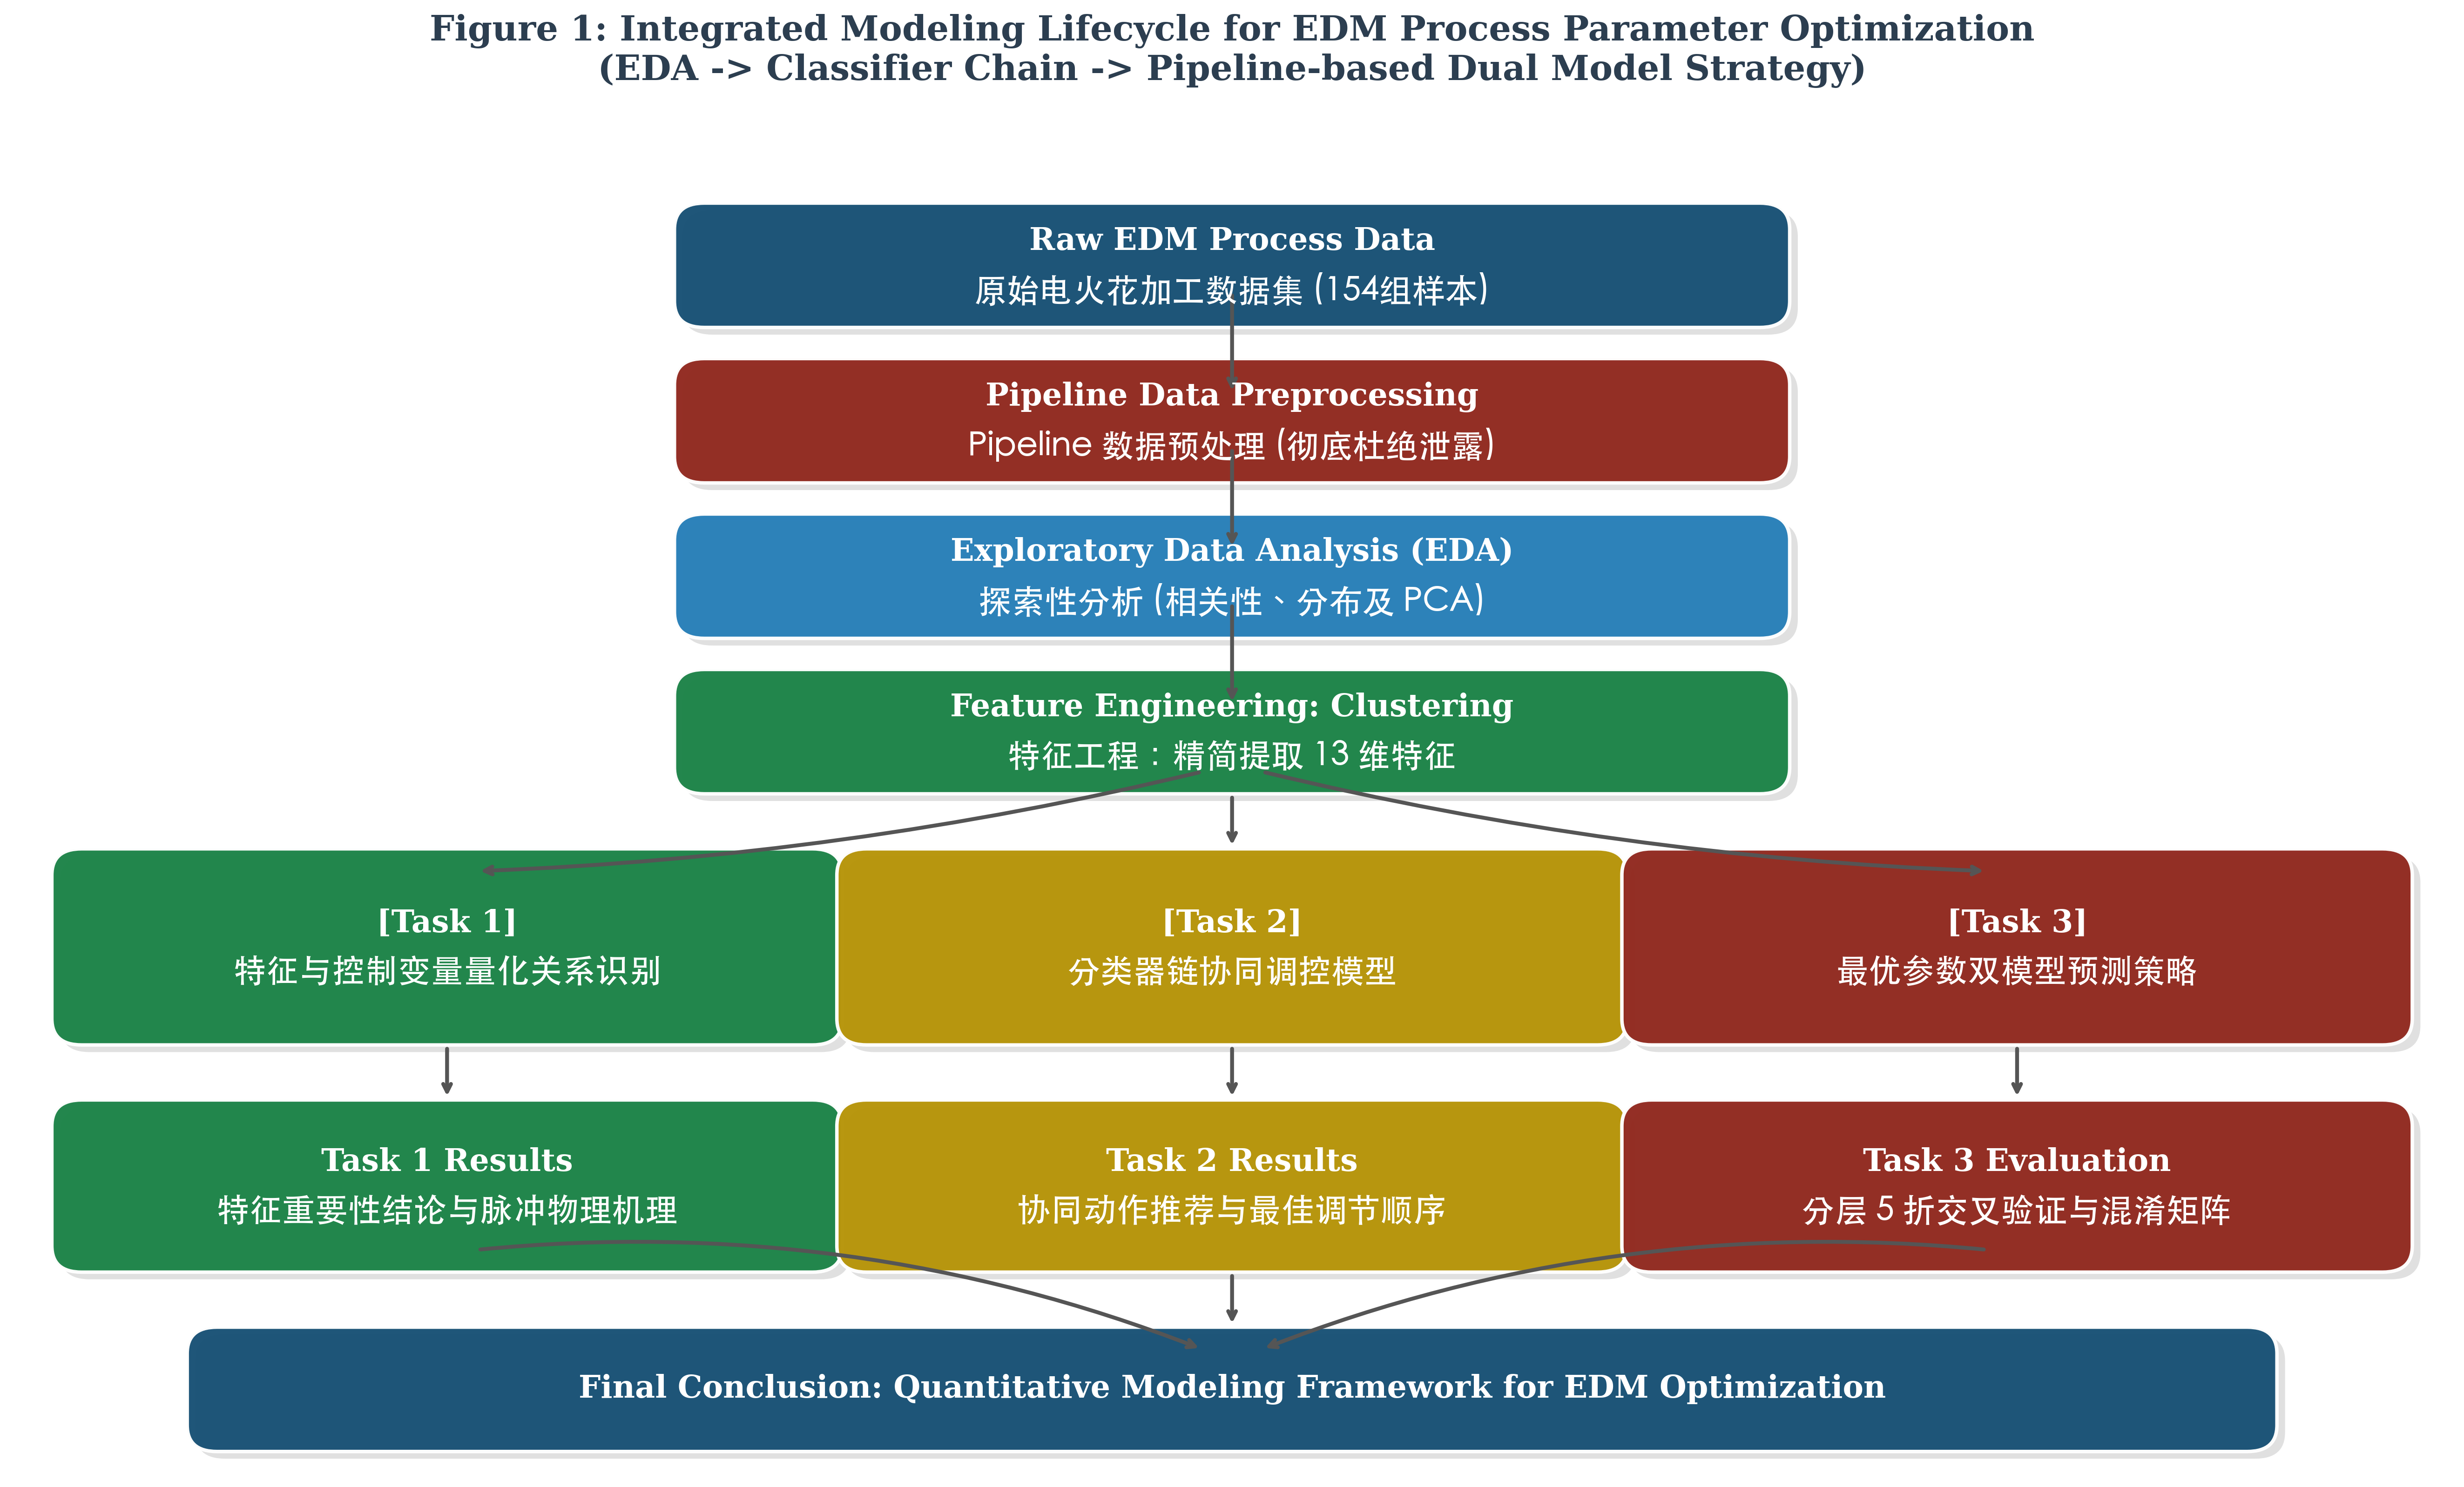
\includegraphics[width=0.88\textwidth]{outputs/Fig12_Flowchart.png}
\caption{电火花加工参数优化的总体建模流程。流程包括特征关系识别、分类器链联合控制建模、双模型参数预测以及特征聚类闭环验证。}
\label{fig:flowchart}
\end{figure}

\section{问题分析}

问题一属于特征—控制变量关系识别问题。由于16个脉冲特征之间存在明显共线性，仅依靠单一线性指标难以完整反映其作用机制，因此需要同时采用线性统计方法和非线性重要性评估方法，识别关键特征并为后续建模提供依据。

问题二属于联合控制决策问题。DFlow 与 DGap 从数值上看并不呈线性相关，但其联合状态分布并非独立，这意味着二者之间存在结构性约束。若仍将两者独立建模，就无法利用这种约束；若直接构造线性叠加指标，又会带来物理解释不足的问题。因此，更合理的思路是从联合概率分解出发进行链式建模。

问题三属于多类别监督学习问题。由于 DFlow 的样本分布极端不均衡，准确率会对主类产生偏置，因此模型比较应以对少数类更敏感的 Macro-F1 作为核心指标，并采用分层5折交叉验证保证评估公平性。

据此，本文采用如下技术路线：
\begin{enumerate}[label=(\arabic*),leftmargin=2em]
\item 用 Pearson 相关分析和随机森林重要性识别关键特征；
\item 用 PCA、LDA 和层次聚类验证特征结构与可分性，并形成“降维分析—建模决策”闭环；
\item 用分类器链建立 DFlow 与 DGap 的联合控制模型；
\item 用 Pipeline 比较五类候选模型，分别确定 DFlow 与 DGap 的最优预测器。
\end{enumerate}

\section{模型假设}

在建立数学模型时，合理的假设是简化实际工程问题并保证模型可解的前提\upcite{ref1}。为保证建模的可实施性，作如下假设：
\begin{enumerate}[label=(\arabic*),leftmargin=2em]
\item 154组样本来自相近加工条件，样本之间可视为相互独立；
\item 16个脉冲特征能够有效刻画放电过程的主要状态\upcite{ref9, ref15}，测量误差对总体结论影响有限；
\item DFlow 与 DGap 的三值编码分别表示“减小/保持/增大”三种离散调节方向；
\item 数据集中的控制标签可视为在当前工况下较优的经验决策结果，因此预测任务可转化为对历史优良控制策略的监督学习；
\item 所得模型适用于与当前数据来源相近的电火花加工工况，不直接外推至材料、电极或工艺条件显著不同的场景。
\end{enumerate}

\section{符号说明}

\begin{table}[H]
\centering
\caption{主要符号及说明}
\label{tab:symbols}
\begin{tabular}{>{\centering\arraybackslash}p{4.5cm}p{9.5cm}}
\toprule
符号 & 含义 \\
\midrule
$n=154$ & 样本总数 \\
$p=16$ & 原始脉冲特征维数 \\
$\bm{X}\in\mathbb{R}^{16}$ & 原始脉冲特征向量 \\
$\bm{X}_{r}\in\mathbb{R}^{13}$ & 层次聚类得到的精简特征向量 \\
$y_f\in\{-1,0,+1\}$ & DFlow 控制变量 \\
$y_g\in\{-1,0,+1\}$ & DGap 控制变量 \\
$r_{x_j,y}$ & 特征与控制变量之间的 Pearson 相关系数 \\
$I_j^{(f)},I_j^{(g)}$ & 特征对 DFlow、DGap 的随机森林重要性 \\
$F_1^{\text{macro}}$ & 宏平均F1分数 \\
$\hat y_f,\hat y_g$ & 模型对 DFlow 与 DGap 的预测值 \\
\bottomrule
\end{tabular}
\end{table}

\section{数据说明与预处理}

\subsection{数据集分布与统计特征分析}

数据集共包含154个样本、18个字段，其中16个为脉冲特征，2个为离散控制变量。类别分布显示：DFlow 的三类样本数为 $5:128:21$，极不均衡；DGap 的三类样本数为 $33:86:35$，相对均衡。该差异意味着 DFlow 的评价更应关注少数类识别能力。

\begin{table}[H]
\centering
\caption{两个控制变量的类别分布}
\label{tab:dist}
\begin{tabular}{cccccc}
\toprule
变量 & 类别$-1$ & 类别$0$ & 类别$+1$ & 总样本数 & 分布特征 \\
\midrule
DFlow & 5（3.2\%） & 128（83.1\%） & 21（13.6\%） & 154 & 极不均衡 \\
DGap  & 33（21.4\%） & 86（55.8\%） & 35（22.7\%） & 154 & 相对均衡 \\
\bottomrule
\end{tabular}
\end{table}

从表\ref{tab:dist} 可以看出，DFlow 的中性状态样本占比超过80\%，因此若模型仅输出类别0就能取得较高准确率，但对实际控制几乎没有意义；DGap 的三类分布则更接近均衡，使其更适合作为标准三分类问题处理。也正因为这一差异，本文在第三问中统一采用 Macro-F1 评价，而不将准确率作为主指标。

16个特征的描述性统计如表\ref{tab:desc} 所示。整体来看，A类均值特征（ASM、ALM）波动较小，而 B、C、I 类中的部分标准差与均值特征具有更大的离散范围，预示着它们更可能携带工况变化信息。

\begin{table}[H]
\centering
\caption{16个脉冲特征的描述性统计}
\label{tab:desc}
\begin{adjustbox}{max width=\textwidth}
\begin{tabular}{ccccc}
\toprule
特征名称 & 均值 & 标准差 & 最小值 & 最大值 \\
\midrule
ASM\_A\_MeanT & -4.656 & 0.111 & -4.960 & -4.380 \\
ASD\_A\_SDevT & 0.070 & 0.066 & 0.000 & 0.390 \\
BSM\_B\_MeanT & 0.816 & 0.328 & 0.040 & 1.140 \\
BSD\_B\_SDevT & 0.115 & 0.112 & 0.000 & 0.450 \\
CSM\_C\_MeanT & 5.462 & 0.313 & 5.100 & 6.100 \\
CSD\_C\_SDevT & 0.108 & 0.101 & 0.000 & 0.380 \\
ISM\_I\_MeanT & 2.188 & 0.546 & 0.810 & 2.910 \\
ISD\_I\_SDevT & 0.230 & 0.188 & 0.000 & 0.770 \\
ALM\_A\_MeanT & -4.653 & 0.077 & -4.850 & -4.500 \\
ALD\_A\_SDevT & 0.097 & 0.054 & 0.010 & 0.260 \\
BLM\_B\_MeanT & 0.843 & 0.258 & 0.270 & 1.140 \\
BLD\_B\_SDevT & 0.199 & 0.133 & 0.000 & 0.470 \\
CLM\_C\_MeanT & 5.454 & 0.258 & 5.120 & 5.870 \\
CLD\_C\_SDevT & 0.188 & 0.110 & 0.000 & 0.370 \\
ILM\_I\_MeanT & 2.260 & 0.394 & 1.070 & 2.790 \\
ILD\_I\_SDevT & 0.396 & 0.211 & 0.030 & 0.940 \\
\bottomrule
\end{tabular}
\end{adjustbox}
\end{table}

在可视化层面，数据总体分布、联合状态频次和各特征在 DGap 三类下的分布图用于说明样本基本面貌。由于该类图更适合作为数据理解的补充证据，本文将其移至附录，仅在后文需要时引用其结论，而将正文篇幅集中用于相关分析、联合决策与预测模型的核心论证。

为保证模型评估的严格性，本文所有性能比较均使用 sklearn 的 Pipeline 将标准化与分类器串联，在每个训练折上单独拟合标准化参数；PCA、LDA 与部分可视化中的全局标准化仅用于分析展示，不参与性能评估。

\begin{figure}[H]
\centering
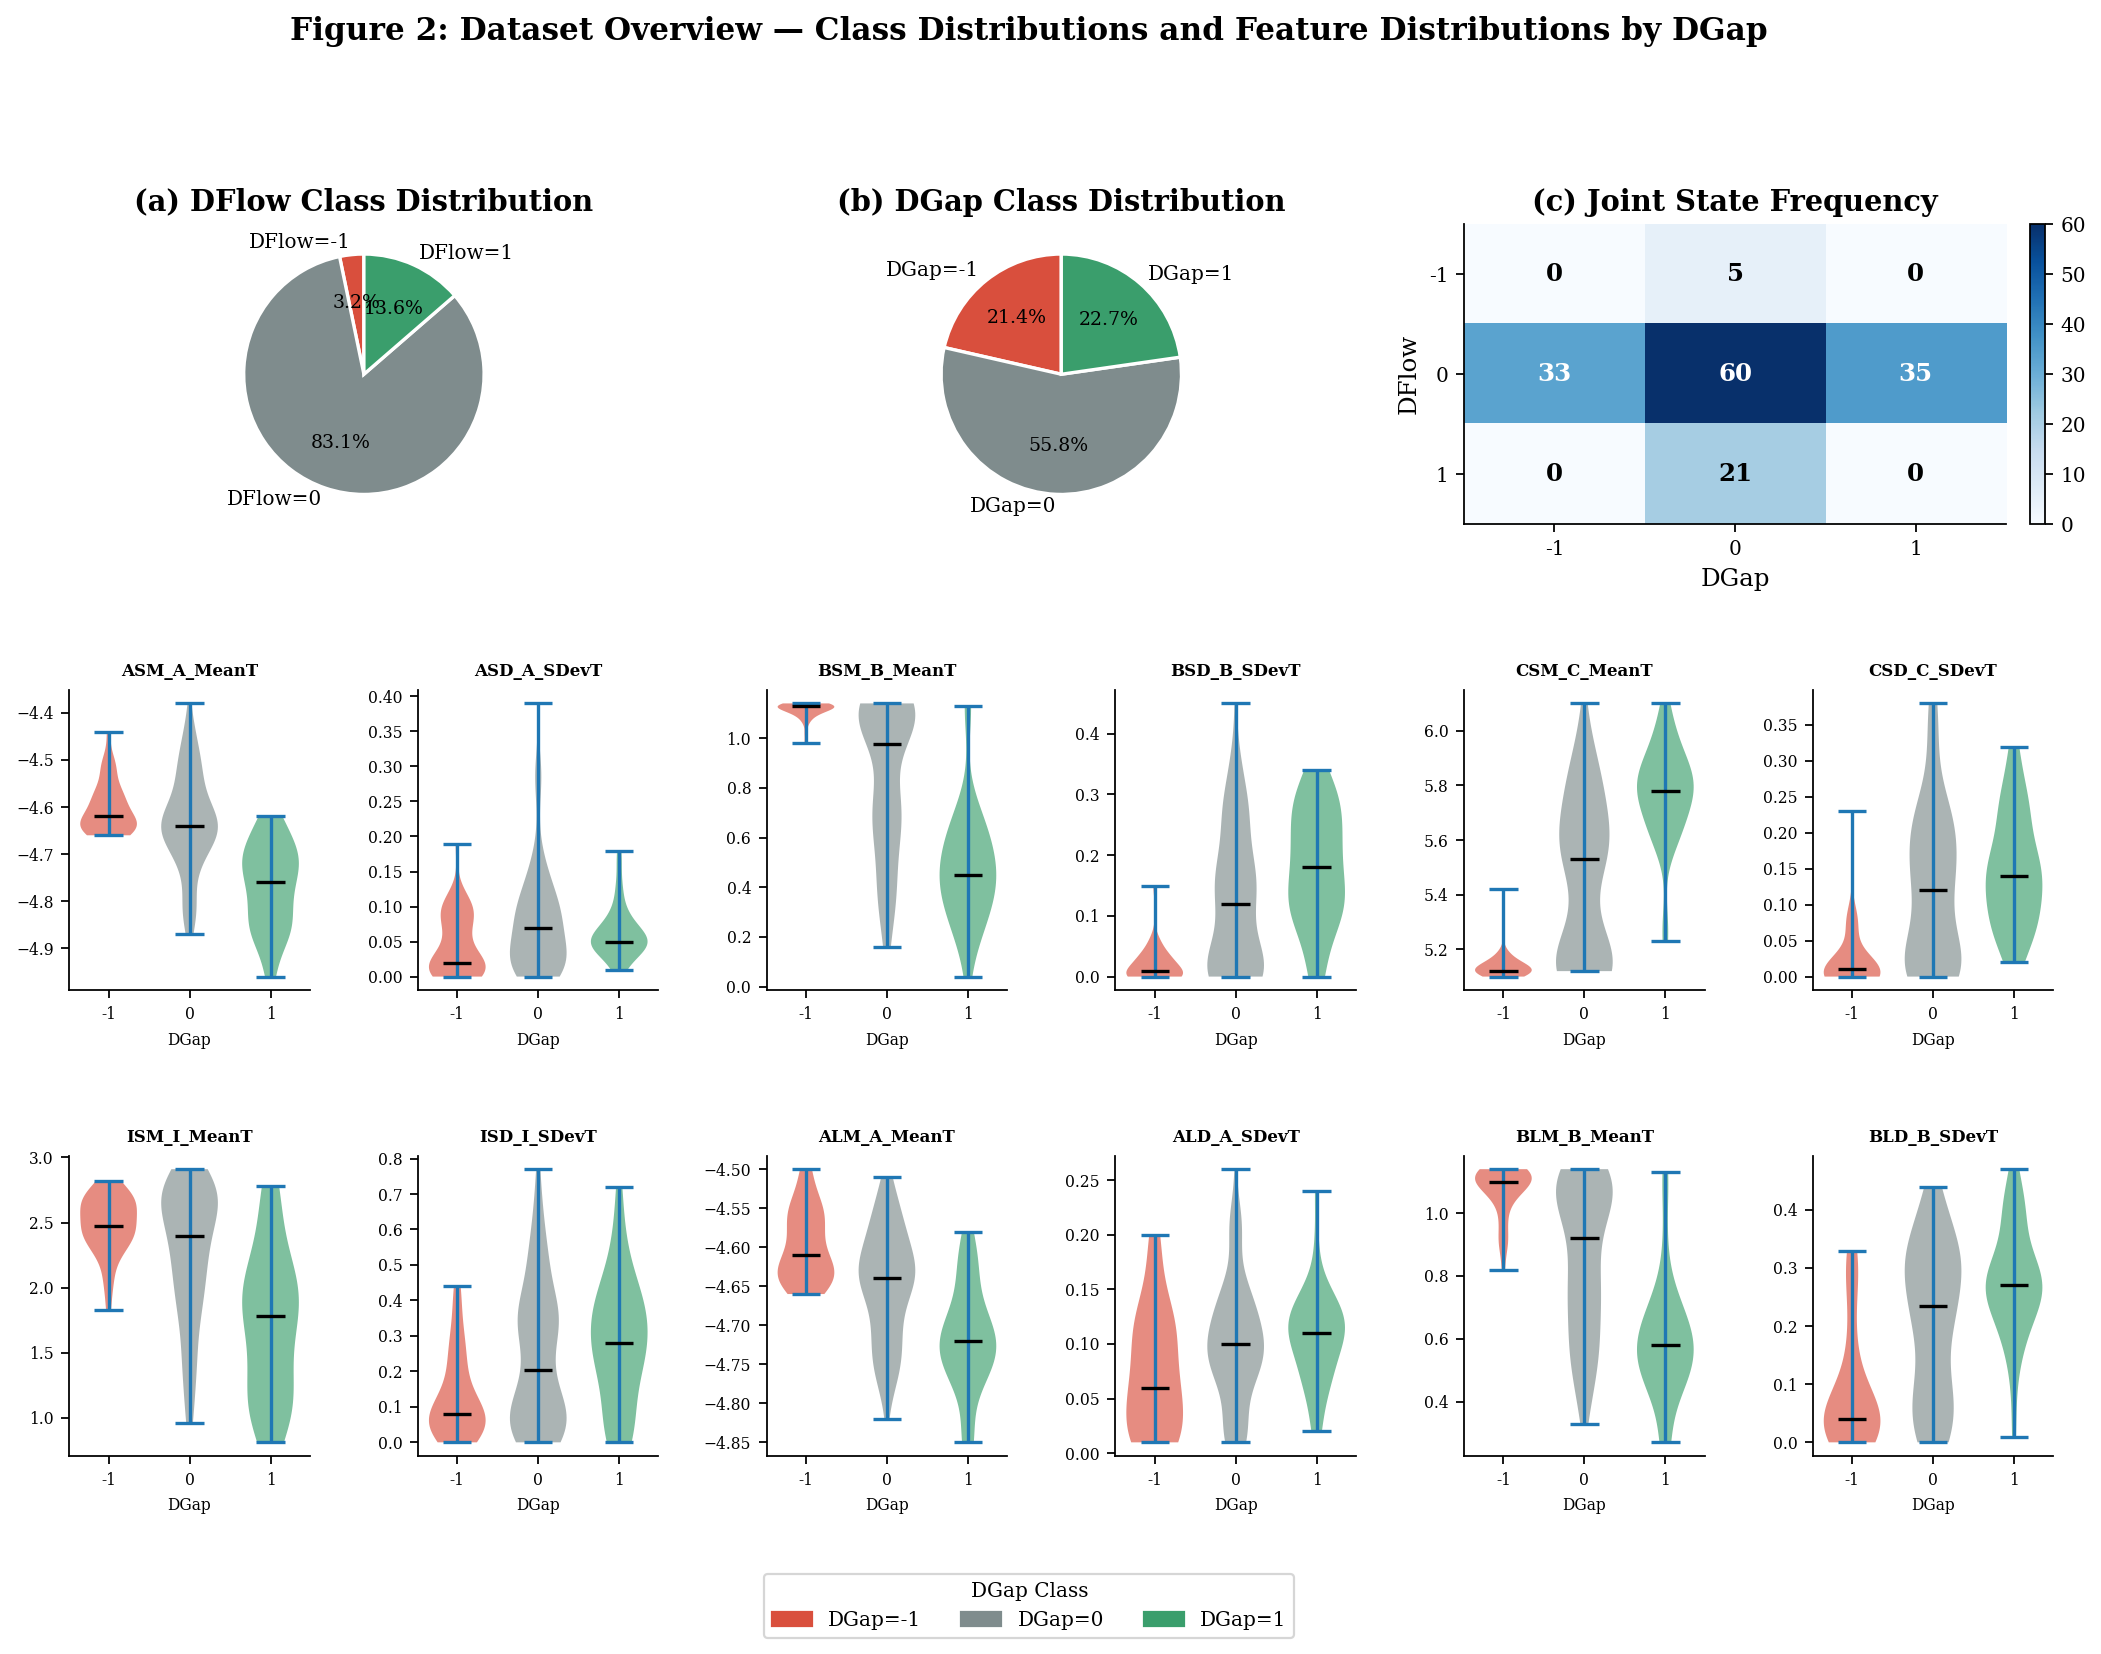
\includegraphics[width=\textwidth]{outputs/Fig1_Data_Overview.png}
\caption{数据集总体分布与特征分布。}
\label{fig:app_data}
\end{figure}

为了更直观地展示样本特征，我们对数据的整体分布进行了可视化分析（如图2所示）。从图2(a)和(b)的类别分布饼图中可以清晰看到，DFlow 处于中性状态（0类）的样本占比高达83.1\%，这一极度的类别不均衡现象直接决定了后续模型评估必须采用对少数类更敏感的 Macro-F1 指标。同时，图2(c)的联合状态热图直观揭示了 DFlow 与 DGap 的“互斥偏移”规律，即两者的非零状态极少同时出现。此外，按 DGap 分组的脉冲特征小提琴图（部分展示）初步印证了不同脉冲特征在不同控制状态下的分布差异，为后续的特征工程提供了先验依据。

\subsection{模型评价指标的数学定义}
鉴于本题控制变量（尤其是 DFlow）存在极度的类别不均衡现象，传统的准确率（Accuracy）容易被多数类主导，无法真实反映模型对少数类（如发生突变的工况）的识别能力。因此，本文选用宏平均 F1 分数（Macro-F1）作为核心评价指标\upcite{ref16}。

根据经典的机器学习评估理论\upcite{ref2}，对于包含 $K$ 个类别的分类任务（本题中 $K=3$，即 $\{-1, 0, 1\}$），首先计算第 $k$ 类的精确率（$Precision_k$）与召回率（$Recall_k$）：
\begin{equation}
    Precision_k = \frac{TP_k}{TP_k + FP_k}, \quad Recall_k = \frac{TP_k}{TP_k + FN_k}
\end{equation}
其中，$TP_k, FP_k, FN_k$ 分别为第 $k$ 类的真正例、假正例和假负例数。由此可得第 $k$ 类的 $F1$ 分数：
\begin{equation}
    F1_k = 2 \times \frac{Precision_k \times Recall_k}{Precision_k + Recall_k}
\end{equation}
最终的 Macro-F1 为所有类别 $F1$ 分数的算术平均值：
\begin{equation}
    Macro\text{-}F1 = \frac{1}{K} \sum_{k=1}^{K} F1_k
\end{equation}
该指标平等地对待每一个类别，迫使模型在追求总体性能的同时，必须兼顾对少数类边界的精准划分。

\section{问题一：脉冲特征与控制变量的量化关系分析}

\subsection{Pearson相关分析}

对全部16个特征分别与 DFlow、DGap 计算 Pearson 相关系数，结果如图\ref{fig:corr} 所示。对 DGap 而言，相关程度最高的三个特征分别为 CSM\_C\_MeanT（0.6693）、BSM\_B\_MeanT（-0.6434）和 CLM\_C\_MeanT（0.6302）；对 DFlow 而言，相关程度最高的特征为 BSD\_B\_SDevT（0.4640）、CLM\_C\_MeanT（0.4508）和 CSD\_C\_SDevT（0.4388）。

这说明 DGap 的变化更容易在脉冲特征中形成稳定、强烈的响应，而 DFlow 的线性可辨性相对较弱，更可能依赖多特征组合关系。为便于与图形证据对应，表\ref{tab:pearson_top} 汇总了两个控制变量上绝对相关系数最大的代表性特征。

\begin{table}[H]
\centering
\caption{Pearson 相关系数排序中的代表性特征}
\label{tab:pearson_top}
\begin{tabular}{lccc}
\toprule
任务 & 特征名称 & 相关系数 & 显著性 \\
\midrule
DGap & CSM\_C\_MeanT & 0.6693 & *** \\
DGap & BSM\_B\_MeanT & -0.6434 & *** \\
DGap & CLM\_C\_MeanT & 0.6302 & *** \\
DFlow & BSD\_B\_SDevT & 0.4640 & *** \\
DFlow & CLM\_C\_MeanT & 0.4508 & *** \\
DFlow & CSD\_C\_SDevT & 0.4388 & *** \\
\bottomrule
\end{tabular}
\end{table}

\begin{figure}[H]
\centering
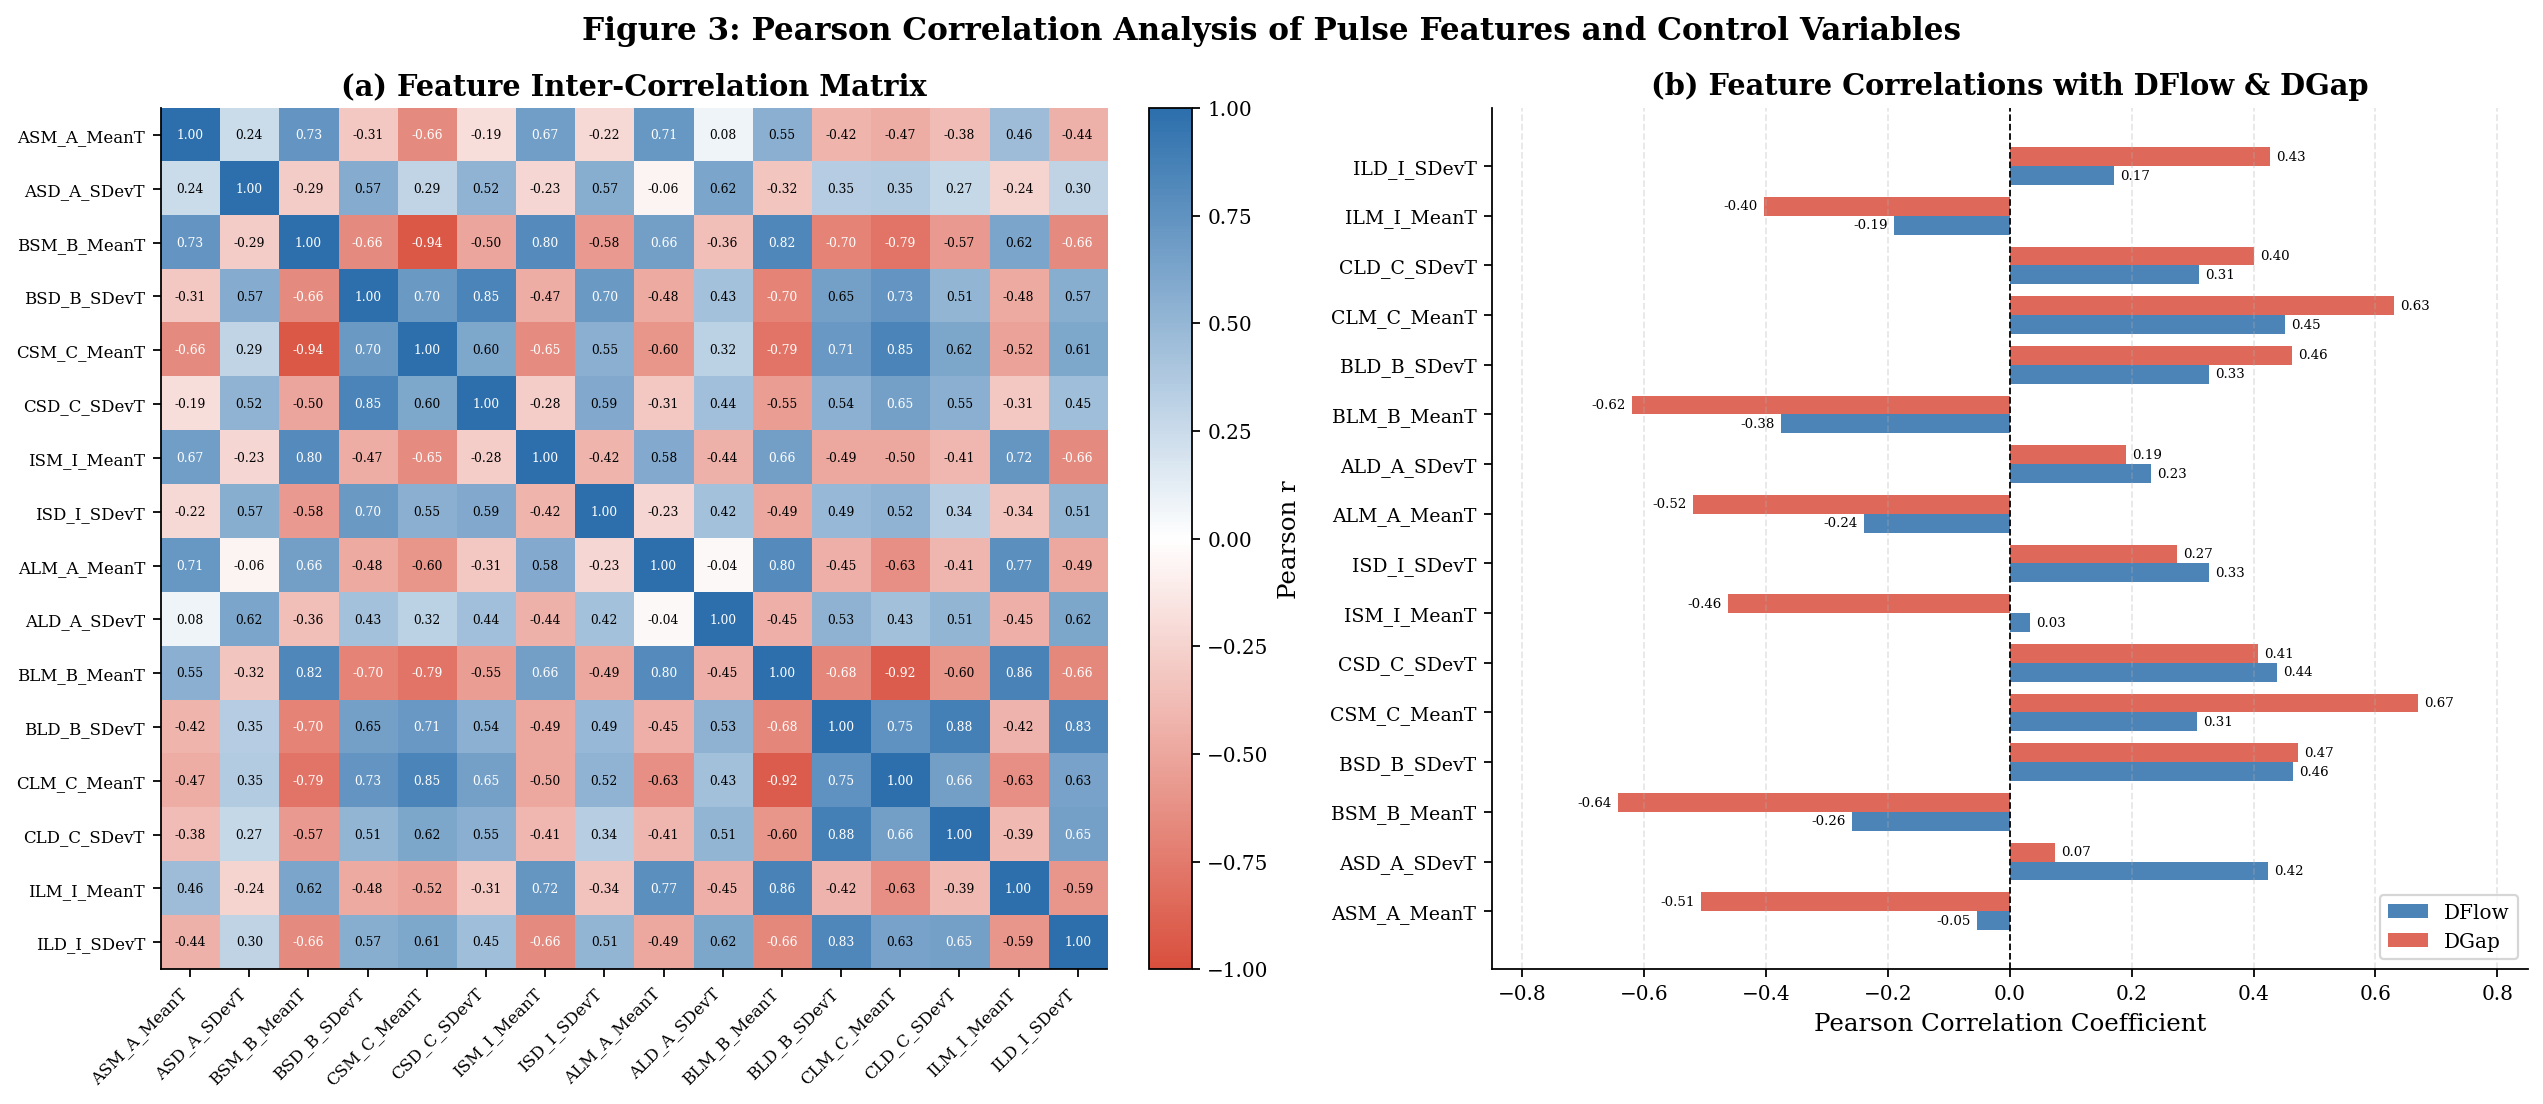
\includegraphics[width=\textwidth]{outputs/Fig2_Correlation_Analysis.png}
\caption{特征相关分析结果。左图为16个脉冲特征的相关矩阵，右图为各特征与 DFlow、DGap 的 Pearson 相关系数。}
\label{fig:corr}
\end{figure}

\subsection{相关结构与显著性解释}

相关分析除了给出排序结果外，还提供了两个对后续建模十分关键的事实。

第一，DGap 的多个核心特征同时表现出较强的方向性：CSM\_C\_MeanT 与 CLM\_C\_MeanT 对 DGap 为显著正相关，BSM\_B\_MeanT 与 BLM\_B\_MeanT 对 DGap 为显著负相关。这意味着在放电间隙增大时，C类脉冲相关时间特征整体上升，而 B 类脉冲相关时间特征整体下降，二者形成了较稳定的“此消彼长”模式。对于 DGap 而言，这类方向一致、强度较大的特征组合有利于模型建立连续且可解释的判别边界。

第二，DFlow 的强相关特征更多集中在标准差类或需通过组合才显现作用的特征上。例如 BSD\_B\_SDevT、CSD\_C\_SDevT 与 CLM\_C\_MeanT 均与 DFlow 显著相关，但单个相关系数的绝对值仍明显低于 DGap 的主导特征。这说明 DFlow 的变化不会像 DGap 那样直接反映为某一类脉冲的单调偏移，而更像是多个脉冲稳定性指标的联合作用结果。因此，DFlow 的建模更依赖能挖掘非线性组合的分类器。

从显著性水平看，16个特征中仅 ASD\_A\_SDevT 对 DGap 的相关性不显著，其余特征几乎全部在 0.05 水平上通过检验；而在 DFlow 侧，仅 ASM\_A\_MeanT 与 ISM\_I\_MeanT 不显著。这说明虽然不同特征的贡献大小存在明显差异，但大多数脉冲特征都携带了一定的控制信息，支持后续使用多变量模型而非单指标阈值模型。

\subsection{随机森林重要性结果的工程含义}

随机森林的重要性排序与线性相关分析既有一致之处，也存在互补信息。对 DGap 而言，两种方法都把 CSM\_C\_MeanT 与 BSM\_B\_MeanT 放在最核心位置，说明 DGap 的主要判别信息既在线性意义下突出，也在非线性模型中保持稳定；这类特征可理解为反映放电间隙状态的“主导型特征”。

对 DFlow 而言，随机森林将 ASM\_A\_MeanT 与 ALM\_A\_MeanT 排在前两位，而 Pearson 相关并未给出同样强烈的信号。这一差异提示：A类脉冲特征对 DFlow 的作用主要通过区间划分或与其他特征的交互触发实现，而不是简单的单调线性关系。换言之，这些特征在某些阈值附近可能具有更强的状态分辨力，因此树模型比线性方法更能挖掘其贡献。

进一步从工程控制角度看，DGap 的重要特征更集中，意味着其调节机制更接近“由少数关键脉冲状态直接驱动”的模式；DFlow 的重要性分布则更分散，反映出流量控制往往服务于排屑、冷却与介质更新等综合效应，需要更多特征共同参与判定。这也为第三问中“DFlow 选用随机森林、DGap 选用 SVM”提供了机制层面的解释：前者更适合复杂交互，后者更适合平滑边界。

\begin{figure}[H]
\centering
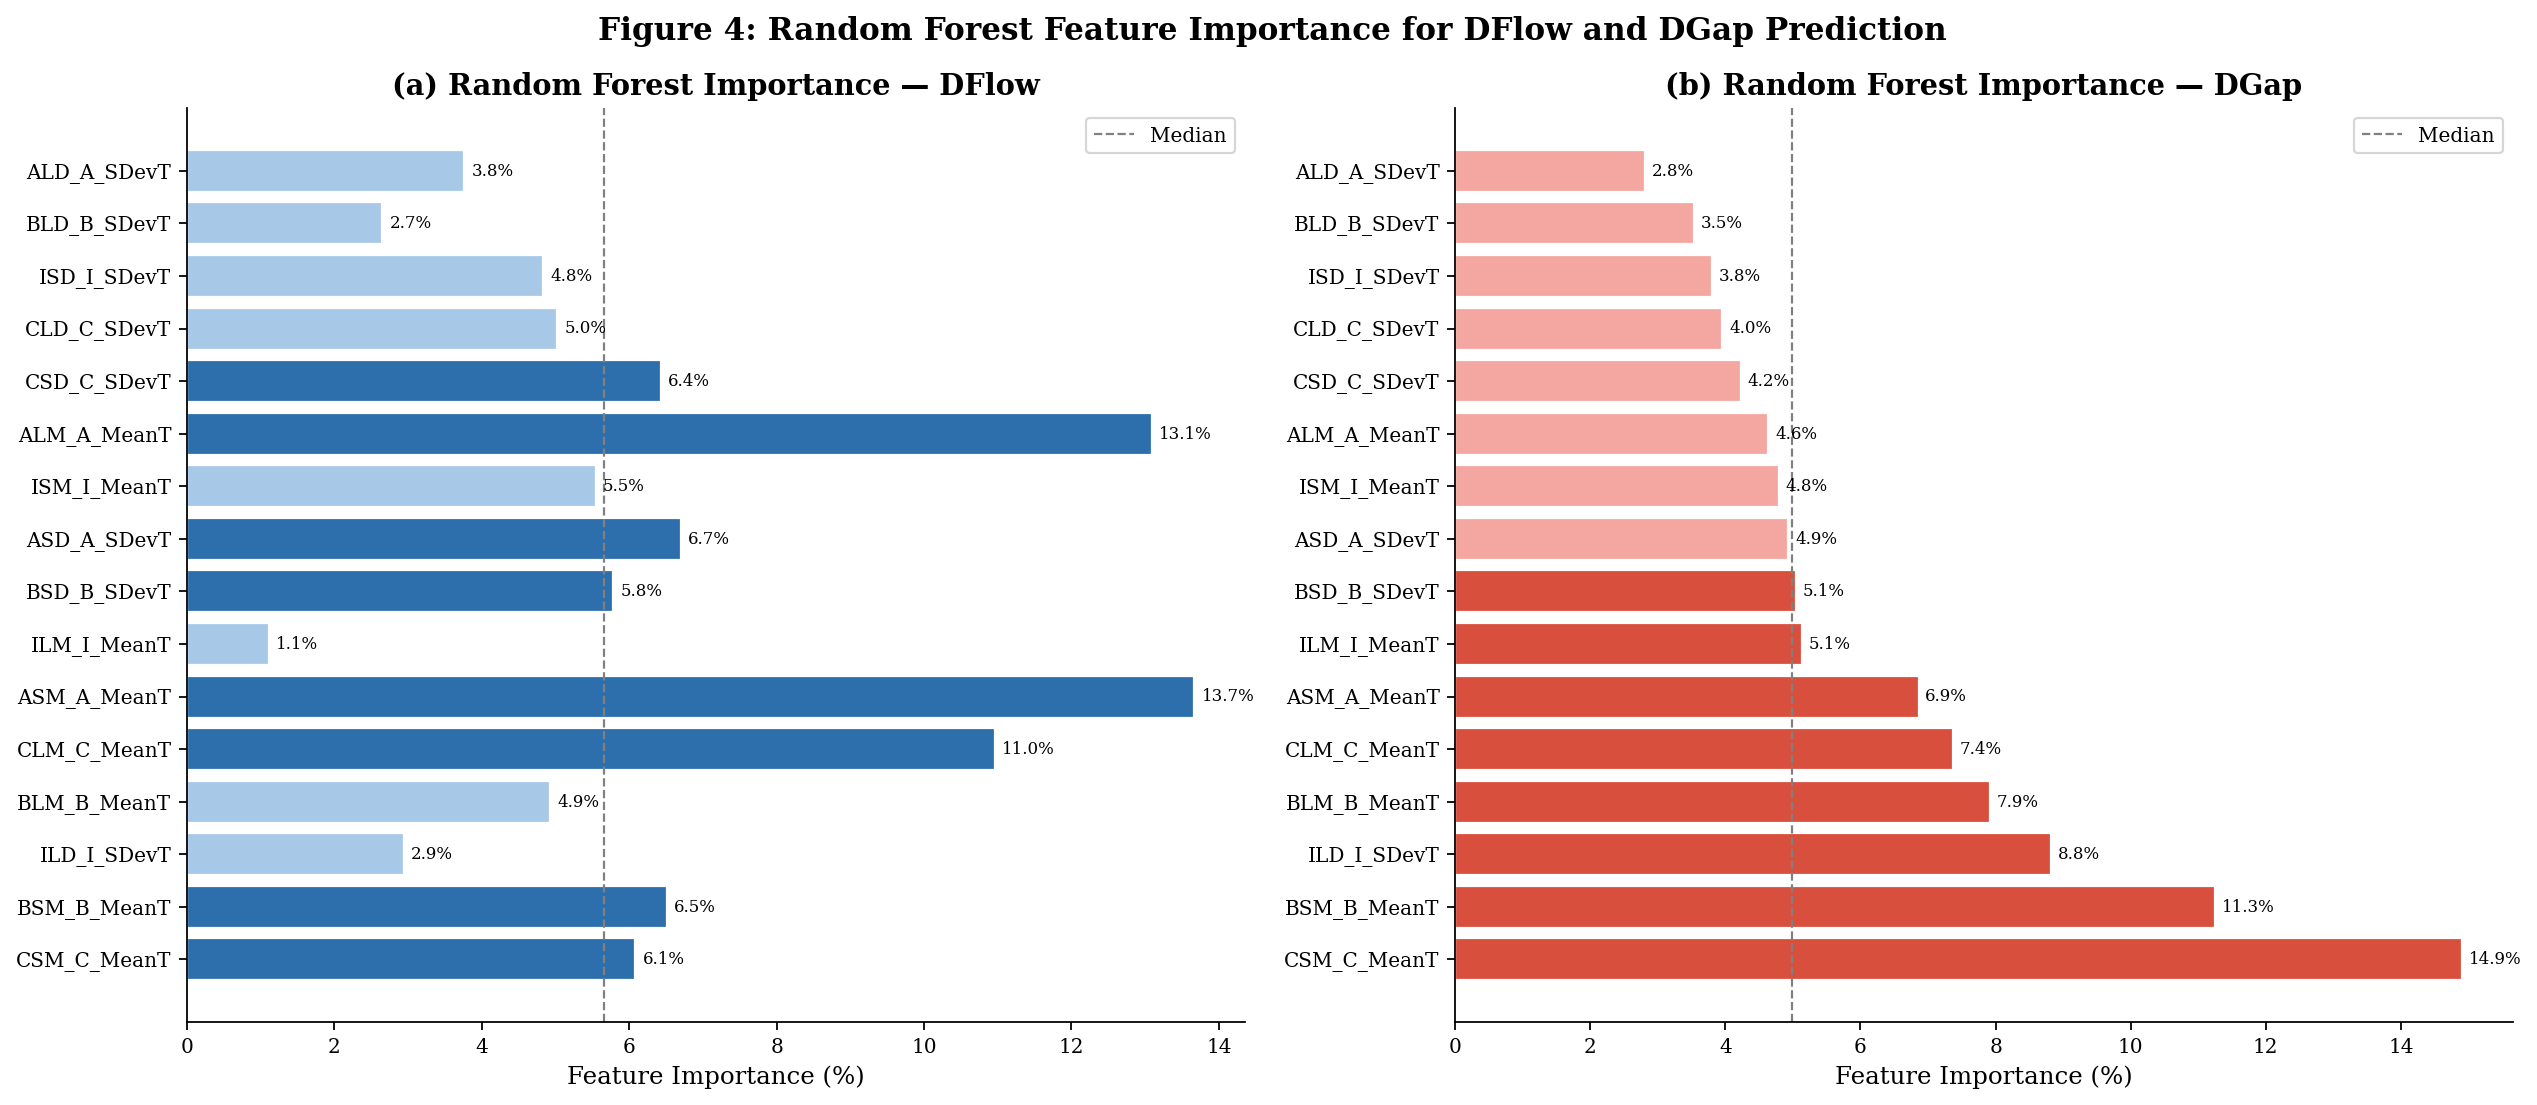
\includegraphics[width=\textwidth]{outputs/Fig4_Feature_Importance.png}
\caption{随机森林特征重要性排序。左图对应 DFlow，右图对应 DGap。}
\label{fig:importance}
\end{figure}

\subsection{降维、判别与特征闭环}

PCA 结果表明前三个主成分累计解释方差为78.07\%，表明大部分信息可由较少维度概括\upcite{ref5}。LDA 投影结果则表明 DGap 在判别空间中呈现较清晰的有序分离\upcite{ref6}，而 DFlow 的难点主要集中在 0 类与 +1 类之间的重叠。相关图形见附录图\ref{fig:app_pca} 与图\ref{fig:app_lda}。

\subsection{PCA、LDA与聚类结果的联合解读}

\begin{figure}[H]
\centering
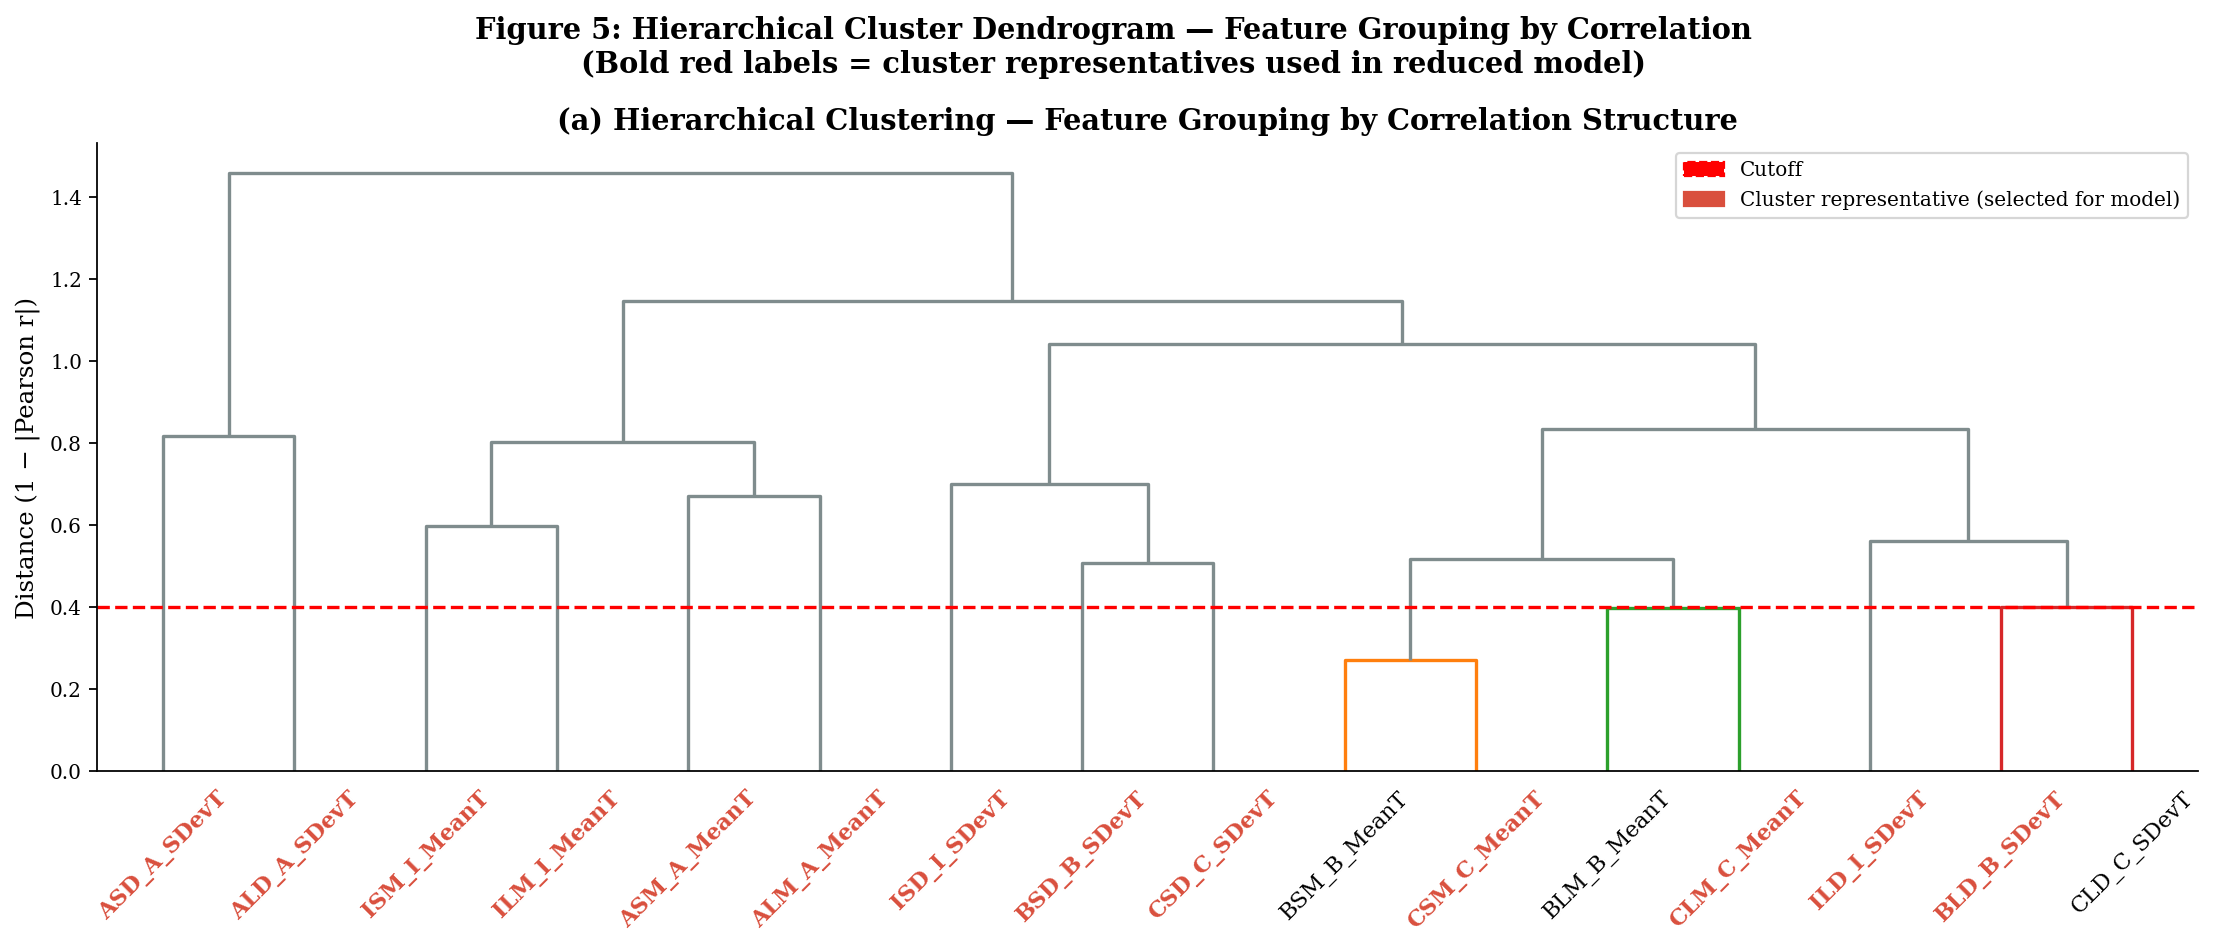
\includegraphics[width=0.92\textwidth]{outputs/Fig11_Dendrogram.png}
\caption{特征相关结构的层次聚类树状图。红色加粗标签为进入精简特征集的代表特征。}
\label{fig:dendrogram}
\end{figure}

\begin{figure}[H]
\centering
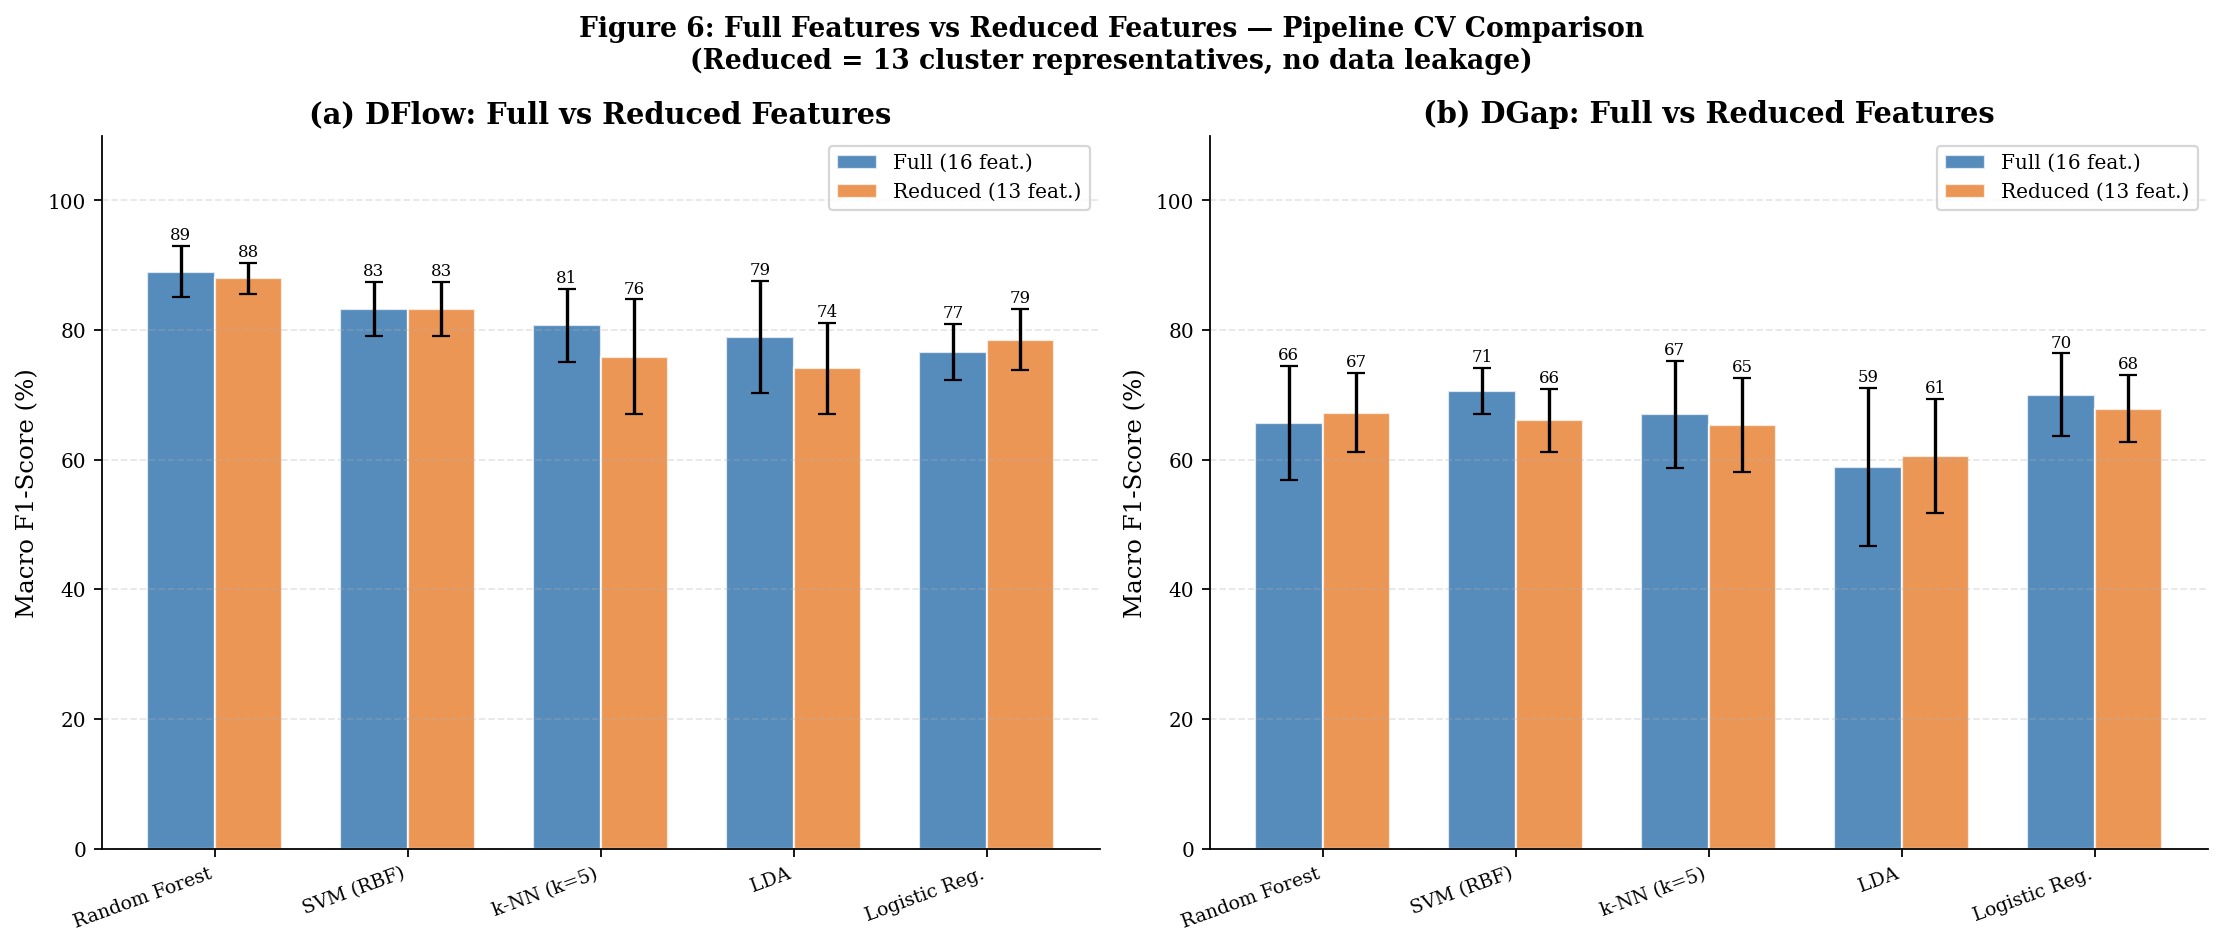
\includegraphics[width=0.92\textwidth]{outputs/Fig7c_Full_vs_Reduced.png}
\caption{全特征与13维精简特征在五类模型上的交叉验证对比。该结果形成“分析冗余—精简建模—性能比较—最终选型”的闭环。}
\label{fig:fullred}
\end{figure}

PCA 与 LDA 的作用并不在于直接替代最终分类器，而在于从几何结构上判断数据是否具备可分性，以及这种可分性主要体现在哪些方向。PCA 的前三个主成分累计解释方差达到78.07\%，说明16维特征中存在较强的低维结构；尤其是第一主成分就解释了57.22\% 的总方差，说明样本变化并非均匀散落在各维度，而是沿某一主方向高度集中。

从 PCA 二维与三维得分图可以看到，DGap 三类样本在 PC1 方向上具有较明显的有序分层，而 DFlow 的类别重叠更强。这一点与前述相关分析高度一致：DGap 的主要判别特征本身就具有较稳定的单调关系，因此更容易在低维投影中保持结构；DFlow 则由于受多特征组合影响，在线性投影空间中难以被完全展开。

LDA 的结果进一步强化了这一认识。DGap 在 LD1 方向上的三个类别均值分别约为 -1.626、-0.096 和 1.770，类别顺序与控制变量编码保持一致，说明脉冲特征中确实含有可直接对应间隙变化方向的判别信息。相比之下，DFlow 的 $-1$ 类在 LD1 上与其他两类显著分离，而 $0$ 类与 $+1$ 类之间距离较近，意味着低流量状态更像一种明显偏离正常加工的特殊状态，而中性与高流量状态之间的边界更依赖非线性细节。

层次聚类的意义在于将上述线性与非线性发现结构化。聚类结果表明，16个特征并非均匀独立，而是可归并为13个特征簇，其中 BSM\_B\_MeanT 与 CSM\_C\_MeanT、BLM\_B\_MeanT 与 CLM\_C\_MeanT、BLD\_B\_SDevT 与 CLD\_C\_SDevT 等高相关对自然聚为同簇。由此得到的13维代表特征既保留了主要判别信息，又压缩了冗余维度。

在获取聚类结构后，对于存在强相关性的特征簇，本文采取的代表特征选取准则是：优先保留与目标控制变量（特别是 DGap）Pearson 相关系数绝对值更大、且在随机森林特征重要性排序中更靠前的特征。例如，在 BSM_B_MeanT 与 CSM_C_MeanT 这对高度负相关的特征中，综合保留判别贡献度更高的 CSM_C_MeanT，从而在消除共线性冗余的同时最大化信息保留率。

但图\ref{fig:fullred} 的结果又表明，精简特征并未在当前样本规模下带来稳定的性能提升。对 DFlow 而言，全特征随机森林为89.0\%，精简特征为88.0\%；对 DGap 而言，全特征 SVM 为70.5\%，精简特征仅为66.1\%。这说明在小样本条件下，某些看似冗余的特征仍可能为模型提供细粒度边界信息，因此本文没有机械地以“降维即更优”为结论，而是保留了更符合数据表现的全特征终模型。

\subsection{精简特征与全特征模型的差异解释}

为更明确说明“为什么分析上发现冗余、最终建模仍保留全特征”这一看似矛盾的问题，表\ref{tab:fullred} 汇总了全特征与13维精简特征在关键模型上的对比结果。可以看出，DFlow 随机森林从89.0\% 下降到88.0\%，差距不大；但 DGap 的 SVM 从70.5\% 下降到66.1\%，下降更明显。这意味着对 DGap 而言，被聚类归并掉的部分特征虽然存在统计相关性，但仍为核方法提供了额外的边界细节。

\begin{table}[H]
\centering
\caption{全特征与13维精简特征的关键模型性能比较}
\label{tab:fullred}
\begin{tabular}{lccc}
\toprule
任务 & 模型 & 全特征 Macro-F1（\%） & 精简特征 Macro-F1（\%） \\
\midrule
DFlow & 随机森林 & 89.0 & 88.0 \\
DGap & SVM（RBF核） & 70.5 & 66.1 \\
DGap & Logistic回归 & 70.0 & 67.9 \\
\bottomrule
\end{tabular}
\end{table}

因此，本文对精简特征集的定位不是“性能更优的终模型”，而是“结构上更紧凑、解释上更清晰的替代方案”。在样本数量进一步增大、噪声更可控或部署端计算资源受限时，13维方案可能更具吸引力；而在当前数据规模下，全特征模型仍是更稳妥的最终选择。

综上，问题一的核心结论是：DGap 对脉冲特征的响应强于 DFlow；C类和B类均值时间特征是两个控制变量的共同敏感区域；A类均值特征对 DFlow 具有重要的非线性贡献；原始特征存在显著冗余，但在当前样本规模下全特征输入仍更有利于最终预测模型性能。

\section{问题二：基于分类器链的协同调控模型}

\subsection{联合结构识别}

DFlow 与 DGap 的联合状态频次如表\ref{tab:joint} 所示。最显著的规律是：当 DFlow 取非零值时，DGap 均为0；反之，当 DGap 取非零值时，DFlow 也均为0。说明二者并非同步增减，而是呈现“互斥偏移”的联合控制结构。

\begin{table}[H]
\centering
\caption{DFlow 与 DGap 的联合频次分布}
\label{tab:joint}
\begin{tabular}{c|ccc|c}
\toprule
\multirow{2}{*}{DFlow} & \multicolumn{3}{c|}{DGap} & \multirow{2}{*}{行合计} \\
\cmidrule(lr){2-4}
& $-1$ & $0$ & $+1$ & \\
\midrule
$-1$ & 0 & 5 & 0 & 5 \\
$0$  & 33 & 60 & 35 & 128 \\
$+1$ & 0 & 21 & 0 & 21 \\
\midrule
列合计 & 33 & 86 & 35 & 154 \\
\bottomrule
\end{tabular}
\end{table}

进一步统计检验表明：Pearson 相关系数为 -0.0051，Spearman 系数为 -0.0069，均不显著；但卡方检验得到 $\chi^2=24.734$、$p=0.0001$，显著拒绝独立性假设。这说明二者不存在简单的线性或单调关系，却存在明确的类别结构依赖。这正是采用联合概率建模而非简单相加的主要依据。

作为辅助性统计证据，本文保留了联合状态图与 Kruskal--Wallis 检验结果，用以说明特征对联合调节状态存在显著区分能力。相关图形见附录图\ref{fig:app_synergy}。该部分主要承担联合结构背景说明的作用，不作为第二问的主模型。
\subsection{分类器链模型建立}

针对联合控制问题，本文引入多标签学习中的分类器链（Classifier Chains）思想\upcite{ref11}。其基本概率分解为
\begin{equation}
P(DFlow,DGap\mid \bm{X})=P(DFlow\mid \bm{X})\cdot P(DGap\mid \bm{X},DFlow).
\label{eq:chain}
\end{equation}

该分解的含义是：先根据脉冲特征预测一级控制变量，再将一级输出与原始特征拼接，作为二级模型的输入，从而将控制变量间的结构依赖显式纳入模型。与将 DFlow 与 DGap 线性相加不同，分类器链不假设二者具有可加的物理量纲，而是直接在条件概率层面刻画联合决策关系，因此更适合本题所呈现的“互斥偏移”数据结构。

在具体算法实现中，该链式分解过程可形式化为两个相继的决策步骤：

\textbf{1. 一级节点决策（针对 DFlow）：}

令原始脉冲特征向量为 $\bm{X} \in \mathbb{R}^d$。一级分类器 $h_1$ 旨在学习从特征空间到 DFlow 状态空间的映射。其决策函数为：
\begin{equation}
    \widehat{DFlow} = h_1(\bm{X}) = \arg\max_{y \in \{-1,0,1\}} P(DFlow = y \mid \bm{X})
\end{equation}

\textbf{2. 二级节点决策（针对 DGap）：}

二级分类器 $h_2$ 的输入不再仅仅是原始特征 $\bm{X}$，而是引入了一级预测结果 $\widehat{DFlow}$ 的增广特征向量 $\bm{X}' = [\bm{X}, \widehat{DFlow}] \in \mathbb{R}^{d+1}$。通过显式地将前一级的决策状态作为先验信息输入，模型能够捕捉到两者在物理工况下的耦合关系。其决策函数表示为：
\begin{equation}
    \widehat{DGap} = h_2(\bm{X}') = \arg\max_{z \in \{-1,0,1\}} P(DGap = z \mid \bm{X}, \widehat{DFlow})
\end{equation}

\textbf{3. 联合推理目标：}

最终，协同调控的最优决策组合 $(\widehat{DFlow}, \widehat{DGap})$ 是通过求解以下联合后验概率最大化问题得到的：
\begin{equation}
    (\widehat{DFlow}, \widehat{DGap}) = \arg\max_{y, z} \left\{ P(DFlow=y \mid \bm{X}) \cdot P(DGap=z \mid \bm{X}, DFlow=y) \right\}
\end{equation}

该数学架构不仅在概率层面保证了逻辑的自洽性，更从特征工程的角度通过“信息传递”解决了传统独立预测模型中存在的状态冲突（Conflict of States）问题。例如，当 $\widehat{DFlow}$ 预测为偏移状态时，模型在第二级推理中会根据条件概率分布，自动抑制 $\widehat{DGap}$ 同时发生偏移的概率，从而在算法底层落实了“互斥偏移”的工艺约束。

在实现上，本文分别评估两种链顺序：
\begin{enumerate}[label=(\arabic*),leftmargin=2em]
\item DFlow $\rightarrow$ DGap：一级用随机森林预测 DFlow，二级用 RBF 核 SVM 在输入中追加一级结果后预测 DGap；
\item DGap $\rightarrow$ DFlow：一级用 RBF 核 SVM 预测 DGap，二级用随机森林在追加一级结果后预测 DFlow。
\end{enumerate}

两种链顺序的比较见图\ref{fig:chain}。结果显示，DFlow $\rightarrow$ DGap 的联合动作 Macro-F1 为70.3\%，略优于反向顺序的69.4\%，因此本文选取前者作为第二问的主模型。其原因在于：DFlow 的一级模型随机森林识别效果更稳定，能够为二级 DGap 模型提供更高质量的条件信息；反向链虽然在一级 DGap 上表现较好，但二级 DFlow 的不均衡问题更明显，导致整体联合动作稳定性下降。

\begin{figure}[H]
\centering
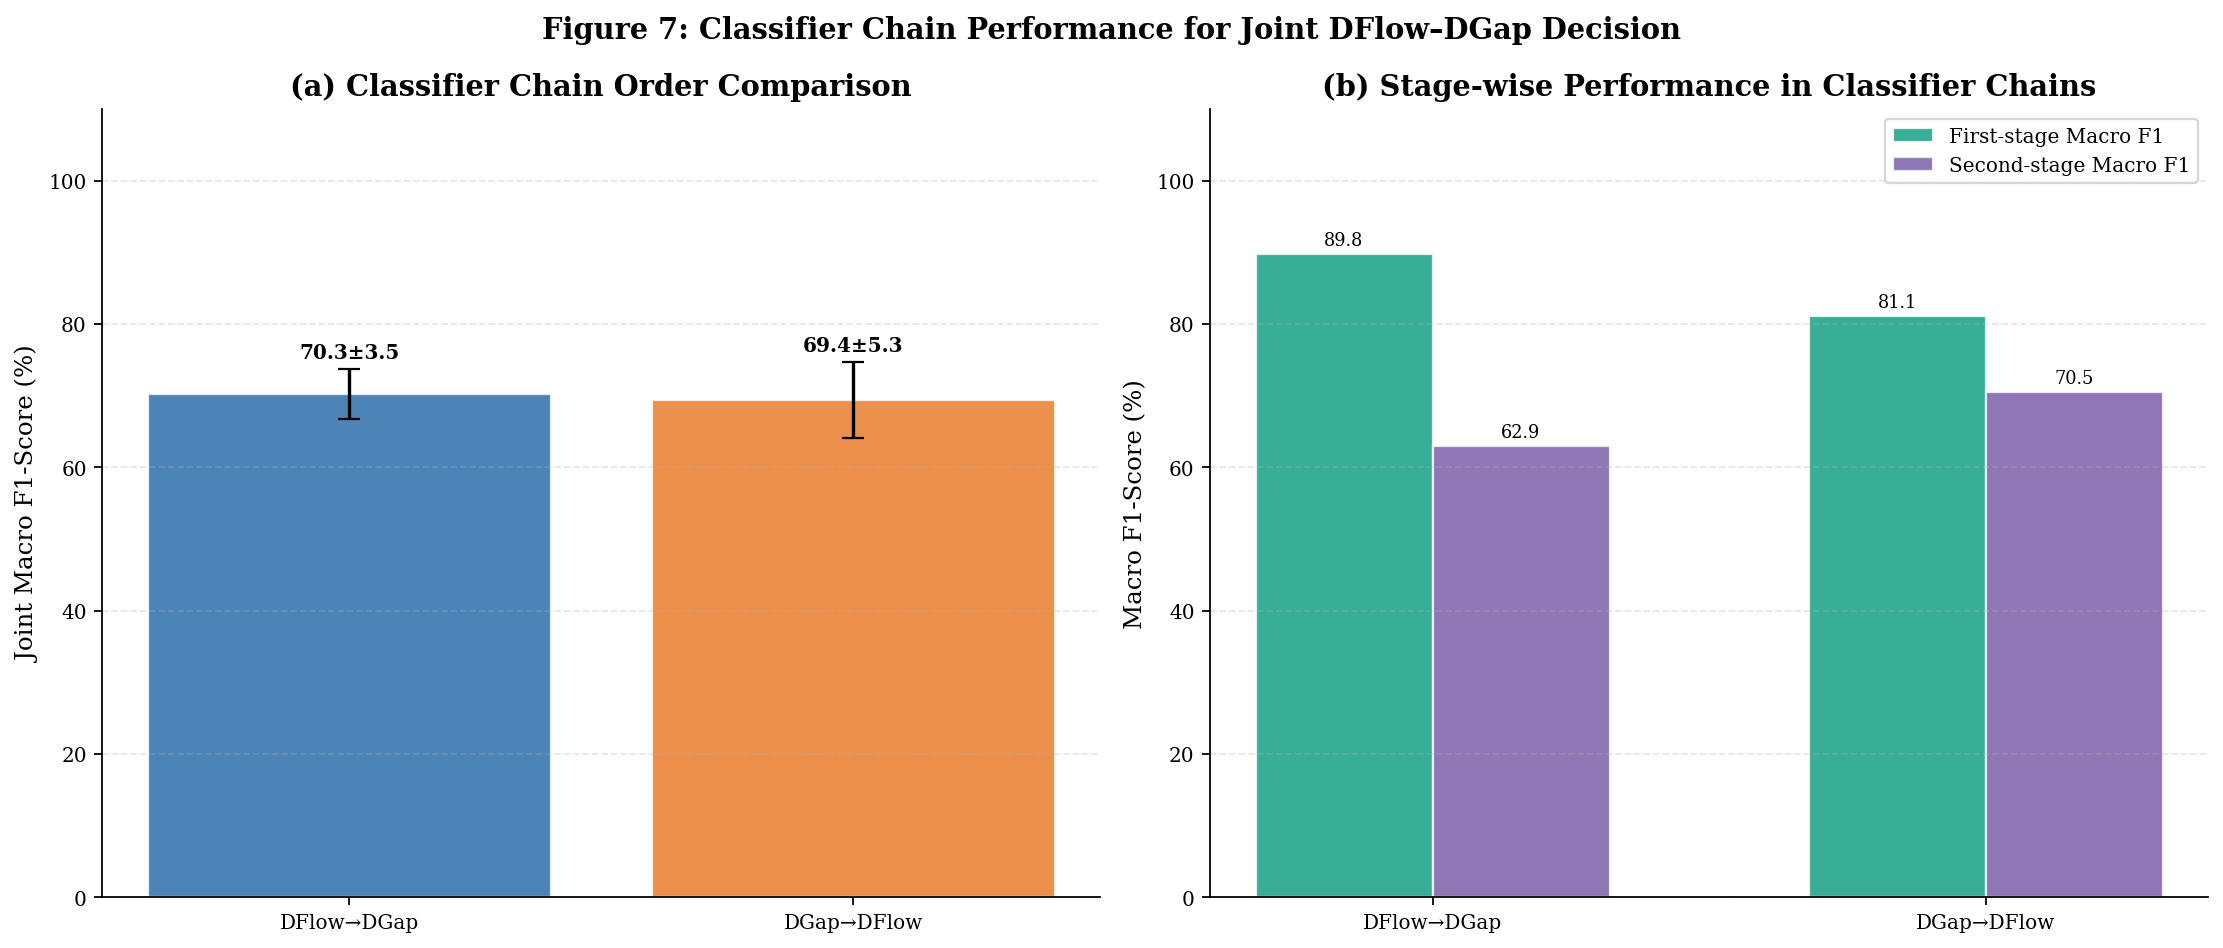
\includegraphics[width=0.92\textwidth]{outputs/Fig8_Classifier_Chain.png}
\caption{分类器链联合决策性能比较。左图为两种链顺序的联合动作 Macro-F1 对比，右图为一级与二级模型的阶段性能。}
\label{fig:chain}
\end{figure}

在测试集上，最优链顺序的联合动作准确率为71.8\%，联合动作 Macro-F1 为78.7\%。这表明分类器链不仅能保持联合动作的结构一致性，还能在小样本条件下给出较为稳定的控制建议。

从阶段性能看，DFlow$\rightarrow$DGap 链中一级 DFlow 模型的 Macro-F1 接近89.8\%，二级 DGap 条件模型的 Macro-F1 为62.9\%。虽然二级性能低于一级，但这种下降是合理的：第二级不仅要识别 DGap 本身，还要在继承一级预测结果的条件下保持联合动作一致性，因此其任务实质上更接近“条件修正”而非独立分类。反向链中，一级 DGap 模型保持在70.5\% 左右，但二级 DFlow 条件模型下降到81.1\%，说明在少数类极度不均衡的条件下，让 DFlow 放在链尾会放大误差传播影响。

此外，从电火花加工的物理机制来看，工作液流量（DFlow）决定了加工区域的宏观流场、冷却条件和排屑能力，这是维持稳定放电的基础环境；而放电间隙（DGap）则是微观层面基于当前宏观环境进行的能量与距离精调。因此，DFlow $\rightarrow$ DGap 的预测链顺序不仅在统计学上能够最小化误差的级联传递，在工程逻辑上也完美契合了“先宏观定环境基调，后微观作精细微调”的加工控制规律。

进一步观察其联合动作意义，可以发现分类器链学到的并非单纯的“两个变量分别预测后碰巧一致”，而是更接近一种工艺决策顺序：先判断当前加工状态是否需要进行明显的流量调节，再在此基础上判断是否需要通过间隙修正完成更细粒度的控制。这一顺序与数据中的联合状态规律相一致，也与现场控制中“先稳住加工状态、再做精细修正”的经验逻辑吻合。

从工程部署角度看，分类器链相比复合指标方案有两个明显优势。其一，链式模型输出的始终是合法的联合动作对 $(\hat y_f,\hat y_g)$，不会因为线性加和而出现不同动作映射到同一编码的混叠问题；其二，链顺序可通过交叉验证数据驱动确定，而不依赖预先假设哪一个变量一定更重要。因此，该方案既保留了统计严谨性，也保留了实际执行层面的可解释性。

\begin{table}[H]
\centering
\caption{分类器链关键性能结果}
\label{tab:chain}
\begin{tabular}{lccc}
\toprule
链顺序 & 联合动作CV Macro-F1（\%） & 联合动作CV标准差 & 测试集联合动作Macro-F1（\%） \\
\midrule
DFlow $\rightarrow$ DGap & \textbf{70.3} & 3.5 & \textbf{78.7} \\
DGap $\rightarrow$ DFlow & 69.4 & 5.3 & -- \\
\bottomrule
\end{tabular}
\end{table}

\begin{table}[H]
\centering
\caption{分类器链输出对应的协同控制建议}
\label{tab:control_rule}
\begin{tabular}{ccc}
\toprule
联合输出 $(\hat y_f,\hat y_g)$ & 控制含义 & 建议动作 \\
\midrule
$(0,0)$ & 工况基本稳定 & 维持当前参数不变 \\
$(+1,0)$ & 流量偏低或排屑不足 & 提高 DFlow，保持 DGap 不变 \\
$(-1,0)$ & 流量偏高或冲刷过强 & 降低 DFlow，保持 DGap 不变 \\
$(0,+1)$ & 间隙偏小或需增强放电间隙 & 提高 DGap，保持 DFlow 不变 \\
$(0,-1)$ & 间隙偏大或需收紧放电间隙 & 降低 DGap，保持 DFlow 不变 \\
\bottomrule
\end{tabular}
\end{table}

据此，本文提出如下协同调控规则：先用分类器链输出联合动作 $(\hat y_f,\hat y_g)$，再据此形成控制建议。若预测结果为 $(0,+1)$ 或 $(0,-1)$，说明当前应优先调节放电间隙；若预测结果为 $(+1,0)$ 或 $(-1,0)$，说明当前应优先调节工作液流量；若预测结果为 $(0,0)$，则维持当前工况。由于分类器链本身已编码联合约束，因此不会像简单线性叠加那样产生状态混叠问题。

\subsection{其他可选方案的简要比较}

除分类器链外，还考虑了两类候选方案：
\begin{enumerate}[label=(\arabic*),leftmargin=2em]
\item \textbf{GMM 状态机方案：}先用高斯混合模型对加工状态聚类，再建立“状态—动作”映射。其优点是工业叙事清晰，便于构造专家系统；缺点是需要人为赋予聚类结果物理意义，在当前样本规模下主观性较强。
\item \textbf{贝叶斯网络方案：}通过概率图模型刻画特征、DFlow 与 DGap 的联合分布。其优点是理论上更严谨，能够直接进行后验推断；缺点是在小样本、高维条件下结构学习与条件概率估计不够稳定，实现与解释成本较高。
\end{enumerate}

综合可实现性、统计稳健性和论文表达的清晰度，分类器链是当前数据条件下的最优方案，因此被选为第二问主模型。

\section{问题三：最优参数预测模型的建立与评价}
\label{sec:model}

\subsection{候选模型与评价准则}

本文选取了机器学习领域\upcite{ref2}最具代表性的五类分类器进行比较，即：随机森林、RBF 核 SVM、k近邻、LDA 和 Logistic 回归模型。由于 DFlow 的类别严重不均衡，若仅看准确率，则模型会偏向预测多数类，因此统一采用 Macro-F1 作为核心评价指标：

对于包含 $K$ 个类别（本题 $K=3$）的分类任务，首先基于混淆矩阵计算第 $k$ 类的精确率 $P_k$ 与召回率 $R_k$：
\begin{equation}
    P_k = \frac{TP_k}{TP_k + FP_k}, \quad R_k = \frac{TP_k}{TP_k + FN_k}
\end{equation}
其中，$TP_k$（真正例）、$FP_k$（假正例）和 $FN_k$（假负例）分别表示第 $k$ 类被正确预测、误判为第 $k$ 类以及漏判的样本数。

在此基础上，Macro-F1 定义为各类别 F1 分数的调和平均再取算术平均：
\begin{equation}
    F_1^{\text{macro}} = \frac{1}{K} \sum_{k=1}^{K} \frac{2 P_k R_k}{P_k + R_k}
\end{equation}
该指标平等地对待每一个类别，迫使模型在追求总体性能的同时，必须兼顾对少数类边界的精准划分。

此外，为保证后续模型评估的严格性，所有模型均在 \texttt{sklearn.pipeline.Pipeline} 中完成数据标准化与分类器拟合，并使用分层 5 折交叉验证（Stratified 5-Fold CV）。这一设定确保了标准化参数仅在训练折上计算，使得不同模型的性能比较建立在完全无数据泄露（No Data Leakage）的同一评估框架下\upcite{ref10}。

\subsection{交叉验证结果与模型选取}

交叉验证结果如表\ref{tab:cv} 和图\ref{fig:modelperf} 所示。DFlow 预测中，随机森林以89.0\% 的 Macro-F1 排名第一；DGap 预测中，RBF 核 SVM 以70.5\% 的 Macro-F1 排名第一。说明两个控制变量对应的最优分类器并不相同：DFlow 更依赖非线性树模型对复杂边界的划分能力，DGap 则更适合由核方法刻画相对平滑的判别边界。

\begin{table}[H]
\centering
\caption{五类模型的5折交叉验证 Macro-F1 比较（全特征）}
\label{tab:cv}
\begin{tabular}{lcccc}
\toprule
模型 & DFlow F1均值（\%） & DFlow标准差 & DGap F1均值（\%） & DGap标准差 \\
\midrule
随机森林 & \textbf{89.0} & 3.9 & 65.6 & 8.8 \\
SVM（RBF核） & 83.3 & 4.1 & \textbf{70.5} & \textbf{3.5} \\
k-NN（k=5） & 80.7 & 5.6 & 67.0 & 8.2 \\
LDA & 78.9 & 8.7 & 58.9 & 12.3 \\
Logistic回归 & 76.6 & 4.3 & 70.0 & 6.3 \\
\bottomrule
\end{tabular}
\end{table}

\begin{figure}[H]
\centering
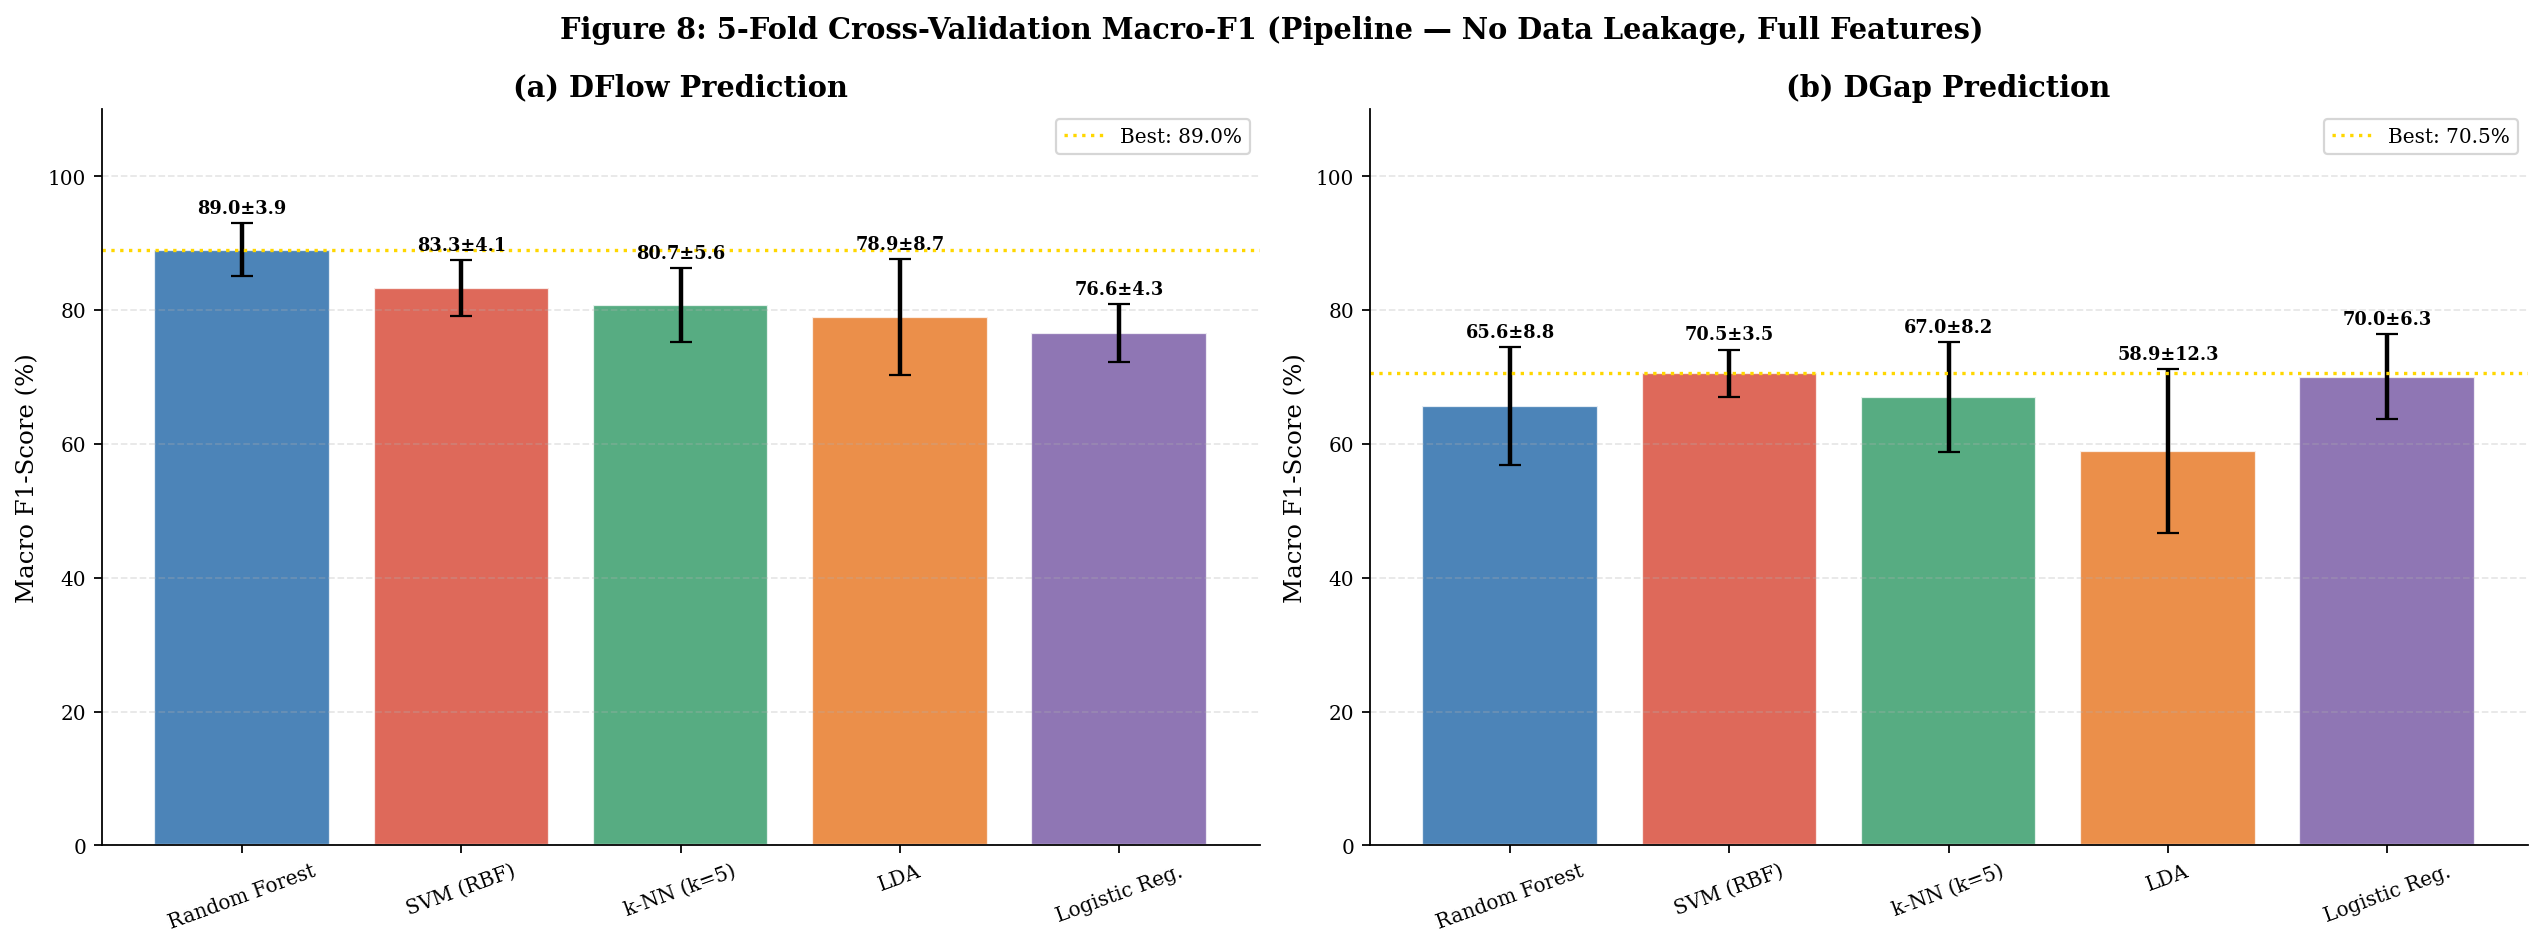
\includegraphics[width=0.96\textwidth]{outputs/Fig7_Model_Performance.png}
\caption{五类模型在 DFlow 与 DGap 预测上的交叉验证 Macro-F1 比较。}
\label{fig:modelperf}
\end{figure}

\subsection{交叉验证结果的进一步讨论}

从表\ref{tab:cv} 可以进一步看出，不同模型在两个任务上的优劣并不一致，这恰恰说明将 DFlow 和 DGap 强行纳入同一种预测器并不合理。对 DFlow 而言，随机森林明显优于其余模型，且标准差仅为3.9，说明该模型既能捕捉类别不平衡下的复杂边界，又具有较好的折间稳定性。相比之下，k-NN 与 LDA 的波动较大，反映出它们对局部样本分布与线性判别假设更为敏感\upcite{ref3}。

对 DGap 而言，SVM 与 Logistic 回归的表现最接近，分别为70.5\% 和70.0\%。这说明 DGap 的可分结构一方面具有一定的线性趋势，另一方面又存在非线性边界，RBF 核 SVM 正好能够在两者之间取得平衡。而随机森林虽然在 DGap 上仍取得65.6\% 的结果，但其标准差较大，说明不同折叠之间的边界学习稳定性不如 SVM。

给定训练集 $\{(\mathbf{x}_i, y_i)\}_{i=1}^n$，SVM 通过引入径向基核函数（RBF）隐式计算高维内积：
\begin{equation}
    K(\mathbf{x}_i, \mathbf{x}_j) = \exp \left( -\gamma ||\mathbf{x}_i - \mathbf{x}_j||^2 \right)
\end{equation}
最终得到的决策函数 $f(\mathbf{x}) = \text{sgn} (\sum \alpha_i y_i K(\mathbf{x}_i, \mathbf{x}) + b)$ 具有良好的局部平滑性\upcite{ref4}。这种平滑性在物理上对应了放电间隙与极间电场强度的连续演变过程。相比之下，随机森林虽然在 DGap 上取得了 65.6\% 的结果，但由于决策树的阶梯状划分特性，其在处理 DGap 这种具有“连续过渡带”的数据结构时，容易在边界处产生过拟合，导致标准差较大且稳定性不如 SVM。

深究其工程逻辑，工作液流量（DFlow）的控制往往伴随着排屑状态的“突变”（如瞬间短路），这种阈值效应更适合树模型的空间切分；而放电间隙（DGap）带来的脉冲特征演变是一个相对渐进的物理过程，通过 RBF 核函数对支持向量（SV）的局部映射，能更精准地刻画出图 \ref{fig:app_prob} 中所示的 3D 概率曲面。

为避免只给出“最佳模型”而忽略建模取舍，图\ref{fig:modelperf} 与图\ref{fig:fullred} 共同表明：第三问的最终策略不是简单追求单一模型统一全任务，而是在相同预处理框架下分别为两个变量选择更适合其数据结构的模型。这种“同框架、分任务”的建模思路，比统一模型更符合本题两个控制变量的统计特征差异。

\subsection{测试集结果与实际部署含义}

为给出更直观的误差结构，按75\%/25\%划分训练集与测试集，并使用全特征训练最终模型。测试结果见图\ref{fig:cm}。DFlow 的测试集 Macro-F1 为95.8\%，DGap 的测试集 Macro-F1 为64.5\%。需要指出的是，DFlow 测试集中 $-1$ 类仅有1个样本，因此该高分数更适合作为辅助说明，不能替代交叉验证结果作为主结论；相比之下，DGap 的测试分数更能反映其实际分类难度，说明该变量仍存在明显类别重叠。

结合电火花加工的实际动态特性，DGap 中性状态（0类）呈现特征弥散的工程原因在于：当放电间隙处于正常维持状态时，极间介质仍可能发生轻微的短路先兆或局部的拉弧波动，导致此时采集到的脉冲特征（尤其是时间标准差类特征）会自然地向“偏大”或“偏小”类的特征区间溢出。这种固有的动态物理波动性使得静态截面数据难以刻画出绝对清晰的静态边界，这也进一步凸显了在未来研究中引入时序动态特征的必要性。

为了使测试结果更具可读性，表\ref{tab:testbrief} 汇总了两个终模型在测试集上的核心指标。可以看到，DFlow 的准确率和 Macro-F1 都较高，但这部分优势与测试集中样本分布高度偏向中性状态有关；DGap 的准确率仅为64.1\%，而 Macro-F1 为64.5\%，说明其误差在三类之间分布更均匀，也更真实地反映了模型面临的判别难度。

\begin{table}[H]
\centering
\caption{最终双模型在测试集上的核心指标}
\label{tab:testbrief}
\begin{tabular}{lccc}
\toprule
任务 & 模型 & Accuracy（\%） & Macro-F1（\%） \\
\midrule
DFlow & 随机森林 & 97.4 & 95.8 \\
DGap & SVM（RBF核） & 64.1 & 64.5 \\
\bottomrule
\end{tabular}
\end{table}

从部署角度理解，这意味着系统在面对“是否保持当前流量不变”时会表现得更稳健，而在“如何区分三种间隙状态”时仍存在一定模糊带。因此，若未来希望将模型嵌入在线控制系统，一个可行思路是将 DFlow 作为相对稳定的粗调通道，将 DGap 作为需要更频繁更新、更依赖上下文信息的精调通道。这样的解释与第二问中分类器链的协同逻辑也是一致的：先做较稳定的状态判别，再做更细粒度的条件修正。

为了将上述“粗调-精调”协同逻辑进一步严密化，并指导未来的在线系统部署，我们可以将其抽象为引入预测置信度的\textbf{双级递阶控制策略（Two-Stage Hierarchical Control Strategy）}。

设在 $t$ 时刻，系统采集到实时脉冲特征向量 $\mathbf{X}^{(t)}$，模型输出各类别的后验概率分布 $P(\cdot \mid \mathbf{X}^{(t)})$。我们引入信息熵 $H$ 作为预测不确定性（即前文所述“模糊带”）的量化度量：
\begin{equation}
    H(y \mid \mathbf{X}^{(t)}) = - \sum_{k \in \{-1,0,1\}} P(y=k \mid \mathbf{X}^{(t)}) \log_2 P(y=k \mid \mathbf{X}^{(t)})
\end{equation}

由于 DFlow 的宏观预测较为稳健（低熵），而 DGap 的微观预测存在类别重叠（高熵），实际部署时的在线控制律可设计为带置信度阈值的链式状态更新：

\textbf{1. 宏观粗调更新（基于 DFlow）：}
\begin{equation}
    u_{flow}^{(t)} = 
    \begin{cases}
        \arg\max_k P(DFlow=k \mid \mathbf{X}^{(t)}), & \text{if } H(DFlow \mid \mathbf{X}^{(t)}) \leq \tau_{flow} \\
        u_{flow}^{(t-1)}, & \text{otherwise}
    \end{cases}
\end{equation}
其中 $\tau_{flow}$ 为系统设定的刚性熵阈值，当模型置信度不足时保持前一时刻的流量状态，以避免工况基准的频繁震荡。

\textbf{2. 微观精调更新（基于 DGap）：}
在确定 $u_{flow}^{(t)}$ 的基础上，引入平滑因子 $\lambda \in (0, 1]$ 调和历史状态与当前预测：
\begin{equation}
    u_{gap}^{(t)} = \lambda \arg\max_k P(DGap=k \mid \mathbf{X}^{(t)}, u_{flow}^{(t)}) + (1-\lambda) u_{gap}^{(t-1)}
\end{equation}

这一数学表述不仅将统计误差转化为工程上可操作的防抖控制律，也在理论上完美映射了问题二中所构建的条件概率机制。

\begin{figure}[H]
\centering
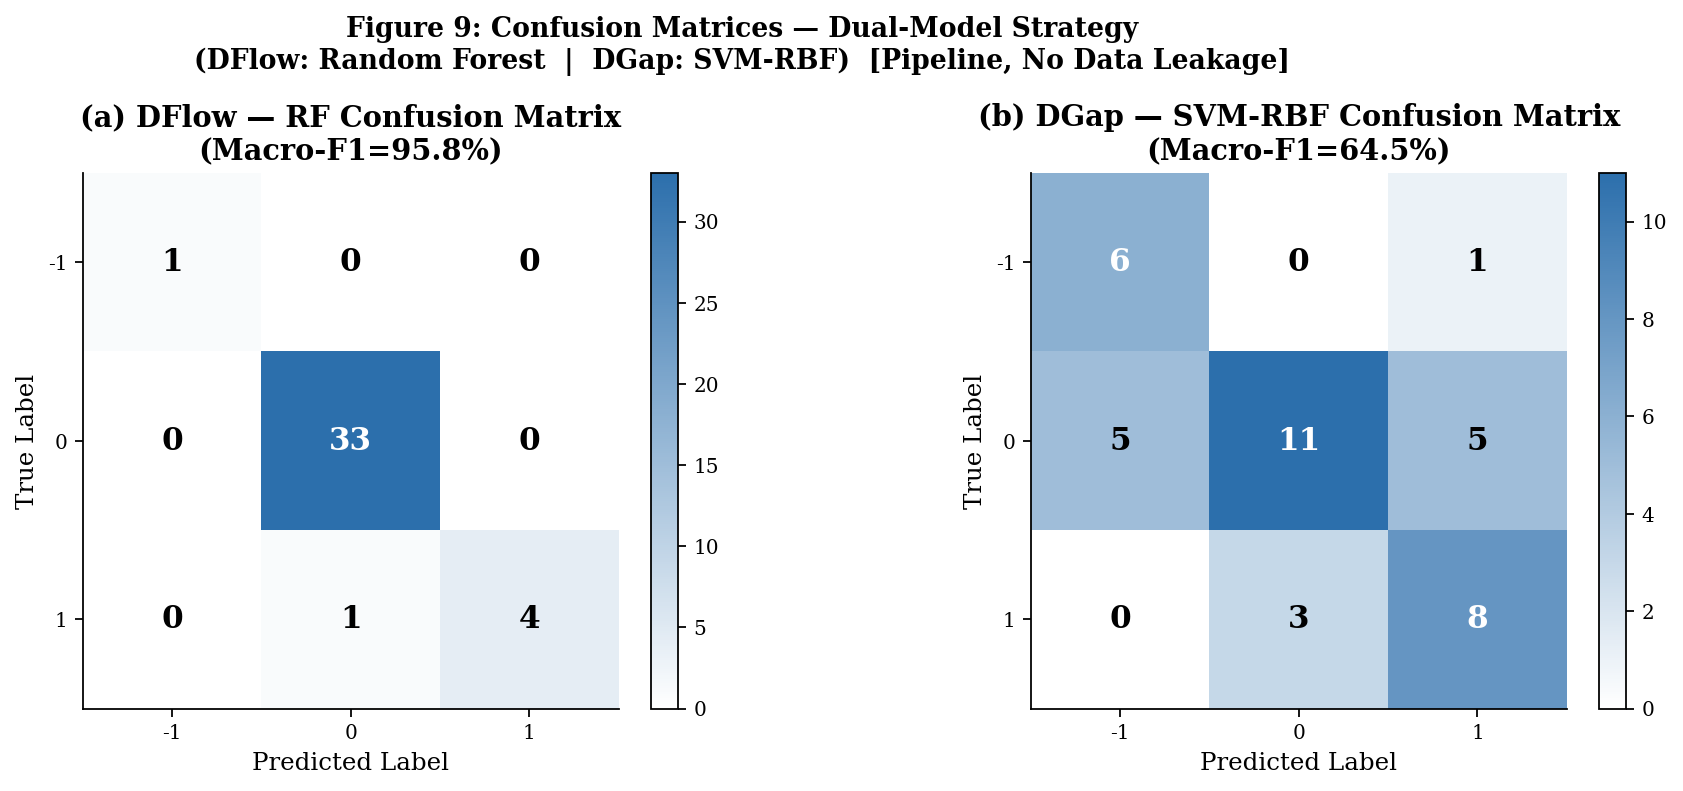
\includegraphics[width=0.92\textwidth]{outputs/Fig8_Confusion_Matrices.png}
\caption{最终双模型策略在测试集上的混淆矩阵。图(a)对应 DFlow 的随机森林模型，图(b)对应 DGap 的 SVM 模型。}
\label{fig:cm}
\end{figure}

为增强可解释性，本文仍保留 DGap 关键特征空间中的决策边界、三维散点图，以及 DFlow 分组箱线图作为补充图形证据。它们主要用于说明分类边界形状、类别重叠位置以及关键特征在不同控制状态下的分布差异，因此统一移至附录展示，正文仅保留其结论性解释。

从这些补充图形可以看出，DGap 的 $-1$ 类与 $+1$ 类在关键特征上分离较明显，而中性状态 0 类分布较为弥散，这正是其分类难度高于 DFlow 的原因之一。与此同时，DFlow 的 A 类均值特征在不同状态下呈现更明显的箱体偏移，这与随机森林重要性排序中 ASM\_A\_MeanT 和 ALM\_A\_MeanT 的领先地位相呼应。相关图形见附录图\ref{fig:app_prob} 以及支撑材料中的其余输出图。


\begin{figure}[H]
\centering
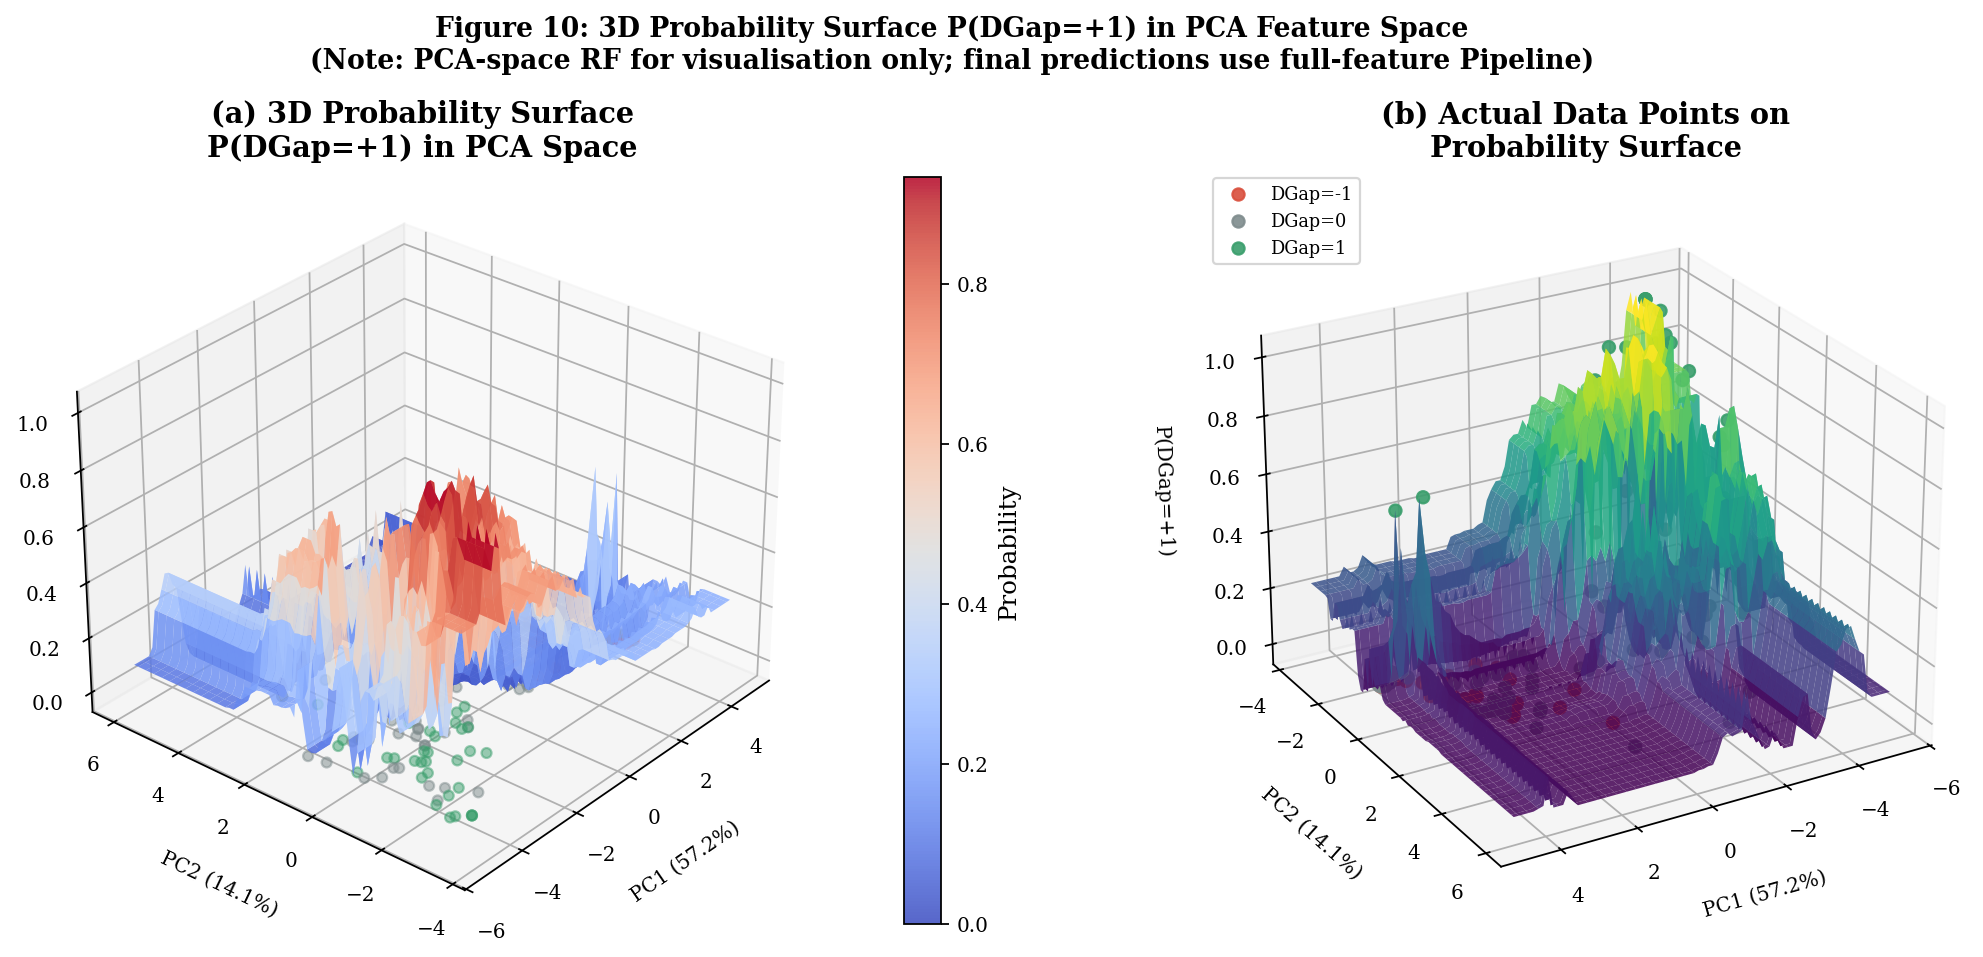
\includegraphics[width=\textwidth]{outputs/Fig14_3D_Probability_Surface.png}
\caption{DGap 概率曲面三维可视化。}
\label{fig:app_prob}
\end{figure}

为进一步提升机器学习预测模型的工程可解释性，我们将高维特征空间投影至 PCA 前两个主成分构建的二维子空间，并绘制了最优模型对 DGap=+1 状态的预测概率三维曲面（如\ref{fig:app_prob}所示）。图中高度（Z轴）及颜色深浅代表模型输出的后验概率大小，散点为真实样本点。可以观察到，高概率区域（深色波峰）与真实 +1 类样本的分布高度重合，而不同类别之间的过渡带呈现出明显的非线性折叠特征。这一拓扑结构直观地解释了为何 RBF 核 SVM 与集成树模型能在该分类任务中显著优于简单线性模型（如 LDA ），证明了本文双模型选型的合理性。

\section{模型评价与推广}

本文模型具有以下优点：
\begin{enumerate}[label=(\arabic*),leftmargin=2em]
\item 采用多种统计与机器学习方法交叉验证，结论一致性较好；
\item 通过层次聚类与全特征/精简特征比较，建立了“发现冗余—比较性能—确定终模型”的完整闭环；
\item 用分类器链替代简单复合指标作为第二问主模型，联合控制的数学表达更严谨；
\item 采用 Pipeline 评估，避免标准化参数泄露；
\item 保留了较多图形证据，使结论更具直观性与说服力。
\end{enumerate}

模型的局限主要包括：
\begin{enumerate}[label=(\arabic*),leftmargin=2em]
\item DFlow 极端不均衡，导致少数类评估存在较大波动；
\item 所有分析基于静态截面数据，尚未纳入时间动态信息；
\item 分类器链虽能刻画联合决策依赖，但其效果仍受一级模型误差传递影响；
\item 结果尚未经过真实闭环加工系统验证，后续需结合在线控制实验进一步检验。
\end{enumerate}

若要面向实际生产部署，还应从样本规模扩充、时序特征引入、传感器噪声鲁棒处理、控制代价约束以及在线模型更新等方面继续完善。

更具体地说，未来改进可以沿三个层面展开。第一，在数据层面，应增加不同材料、不同脉冲参数组合以及不同加工阶段的数据，以降低当前样本分布单一带来的偏差；第二，在模型层面，可考虑引入时间窗口特征、序数分类模型或代价敏感学习，以更精细地处理“相邻状态误判”和“跨级误判”之间的工程差异；第三，在控制层面，可把本文输出的离散动作建议进一步嵌入带约束的闭环控制器中，例如设置调整幅度上限、切换滞回区间以及安全监测门限，使模型建议能够平稳映射到设备执行动作。

此外，本文保留了较多辅助图而非只保留核心图，其目的并非增加展示负担，而是为评审者提供从数据分布、低维结构、联合状态到最终分类边界的完整证据链。对于数模论文而言，这种“主结论+图形旁证”的组织方式有助于增强模型可信度，也便于说明各建模步骤之间的递进关系。

\section{结论}

本文围绕电火花加工中 DFlow 与 DGap 的量化关系识别、协同调控简化与参数预测问题，建立了“特征分析—分类器链—双模型预测”的完整框架。

其主要结论如下：
\begin{enumerate}[label=(\arabic*),leftmargin=2em]
\item 在问题一中，DGap 对脉冲特征的响应更强，CSM\_C\_MeanT、BSM\_B\_MeanT 与 CLM\_C\_MeanT 是最关键的线性敏感特征；随机森林进一步表明，A类均值特征对 DFlow 具有显著的非线性判别作用。
\item 原始16维特征存在9对强相关特征对，经层次聚类可精简为13维代表特征；但在当前小样本条件下，全特征输入的预测性能仍略优于精简特征，因此最终模型仍采用16维输入。
\item 在问题二中，DFlow 与 DGap 虽无线性相关，但联合分布显著不独立。基于此构建的分类器链模型能够更合理地表达联合控制规律，其中 DFlow$\rightarrow$DGap 顺序的联合动作 Macro-F1 为70.3\%，优于反向顺序，适合作为协同调控主模型。
\item 在问题三中，DFlow 的最优预测模型为随机森林，DGap 的最优模型为 RBF 核 SVM；相应的5折交叉验证 Macro-F1 分别为89.0\%和70.5\%。
\end{enumerate}

综上，本文所建模型既给出了脉冲特征与控制变量之间的量化关系，也从联合决策角度提供了可执行的协同控制方案，并形成了可直接服务于实际工艺优化的预测框架。

% ==================== 参考文献 ====================
\begin{thebibliography}{99}
\bibitem{ref1} 姜启源, 谢政, 叶俊. 数学模型（第5版）[M]. 北京: 高等教育出版社, 2018.
\bibitem{ref2} 周志华. 机器学习[M]. 北京: 清华大学出版社, 2016.
\bibitem{ref3} Breiman L. Random Forests[J]. Machine Learning, 2001, 45(1): 5--32.
\bibitem{ref4} Cortes C, Vapnik V. Support-vector networks[J]. Machine Learning, 1995, 20(3): 273--297.
\bibitem{ref5} Jolliffe I T, Cadima J. Principal component analysis: a review and recent developments[J]. Philosophical Transactions of the Royal Society A, 2016, 374(2065): 20150202.
\bibitem{ref6} Fisher R A. The use of multiple measurements in taxonomic problems[J]. Annals of Eugenics, 1936, 7(2): 179--188.
\bibitem{ref7} Kruskal W H, Wallis W A. Use of ranks in one-criterion variance analysis[J]. Journal of the American Statistical Association, 1952, 47(260): 583--621.
\bibitem{ref8} Ho K H, Newman S T. State of the art electrical discharge machining (EDM)[J]. International Journal of Machine Tools and Manufacture, 2003, 43(13): 1287--1300.
\bibitem{ref9} 刘义, 李明, 张涛. 电火花加工过程脉冲分类与状态识别方法研究[J]. 中国机械工程, 2019, 30(12): 1412--1419.
\bibitem{ref10} Pedregosa F, et al. Scikit-learn: Machine learning in Python[J]. Journal of Machine Learning Research, 2011, 12: 2825--2830.
\bibitem{ref11} Read J, Pfahringer B, Holmes G, Frank E. Classifier chains for multi-label classification[J]. Machine Learning, 2011, 85(3): 333--359.
\bibitem{ref12} Yu Y, Dong S, Liu F. A review of advances in electrical discharge machining: From flow field to multi-physics coupled simulations[J]. International Journal of Machine Tools and Manufacture, 2020, 150: 103456.
\bibitem{ref13} Ablyaz T R, Shlykov E S, Muratov K R. Modeling of EDM Process Flushing Mechanism. Materials, 2023, 16(11):4158.
\bibitem{ref14} Goodlet A, Koshy P. Real-time evaluation of gap flushing in electrical discharge machining. CIRP Annals, 2015, 64(1):241–244.
\bibitem{ref15} Dauw D F, Snoeys R, Dekeyser W. Advanced Pulse Discriminating System for EDM Process Analysis and Control. CIRP Annals, 1983, 32(2):541–549.
\bibitem{ref16} Sokolova M, Lapalme G. A systematic analysis of performance measures for classification tasks. Information Processing\& Management, 2009, 45(4):427–437.
\bibitem{ref17} 豆包, 豆包 2.0 专家模型, 北京字节跳动科技有限公司, 2026-04-03.
\bibitem{ref18} 智谱,  GLM-5.0, 北京智谱华章科技有限公司, 2026-04-03.
\end{thebibliography}

% ==================== AI 使用报告 ====================
\section*{AI使用情况报告}

\noindent\textbf{所用AI工具名称和版本：} 
豆包（豆包 2.0 专家模型，使用日期：2026-04-03）
智谱（GLM-5.0，使用日期：2026-04-03）。

\noindent\textbf{具体使用目的和环节：}
\begin{enumerate}[label=(\arabic*),leftmargin=2em]
\item 辅助构建无数据泄露的严密模型评估框架（如基于 sklearn Pipeline 的交叉验证设计）；
\item 辅助探讨多重共线性对不同分类算法的影响，并提供小样本下的特征降维与精简策略参考；
\item 辅助系统性梳理模型的优缺点，并补充将理论预测模型向工业在线部署延伸的工程控制逻辑；
\item 辅助核查学术排版规范、统一图表编号以及优化核心代码的呈现结构。
\end{enumerate}

\noindent\textbf{关键交互记录：}

Q：交叉验证中先全局标准化再划分数据集有什么问题？如何用 sklearn Pipeline 构建无数据泄露的验证框架？

A：先全局标准化会造成数据泄露，测试集的均值、方差信息会提前泄露至训练过程，导致性能评估结果失真。正确方案是用 sklearn Pipeline 将「标准化」与「分类器」完整串联，配合分层 5 折交叉验证，确保每一轮仅在训练折内拟合标准化参数，完全隔离测试集信息，适配类别不均衡场景下的 Macro-F1 指标评估。

\vspace{0.8em}
Q：请梳理我这个数模论文的模型优缺点，以及实际生产应用中需补充的工程因素

A：模型核心优点：多方法交叉验证结论可靠，分类器链协同模型贴合工程实际，双模型策略适配两个控制变量的数据特性，建模逻辑形成完整闭环。局限性：DFlow 少数类样本不足限制泛化能力，静态截面数据未考虑 EDM 加工的时序动态特性，未区分不同误判的工程代价差异，未经过真实闭环系统验证。实际生产需补充：全工况样本库扩充、在线测量噪声鲁棒处理、时序动态模型构建、设备执行约束与安全控制、模型在线更新机制。

\vspace{0.8em}
Q：电火花 B 题的 16 个脉冲特征存在多对强相关特征，多重共线性会对分类模型产生什么影响？有哪些适配小样本场景的处理方法？

A：核心影响：对线性模型（如 Logistic 回归、LDA）会导致参数估计不稳定、系数解释性失效；对树模型、核 SVM 的影响相对较小，但会增加模型计算冗余。适配小样本的处理方法：1. 基于层次聚类做特征精简，从强相关特征簇中选取判别能力最强的代表特征，降维同时最大化信息保留；2. 用 PCA 做特征正交变换，消除共线性，同时保留核心信息；3. 树模型、核 SVM 可保留全特征输入，利用模型自身的抗共线性能力。

\vspace{1.0em}
\noindent\textbf{采纳和人工修改情况：}
AI 工具在数据防泄露框架（Pipeline设计）与特征工程的理论层面提供了有价值的辅助参考。参赛队在此基础上，结合电火花加工的实际物理机理与极度不平衡的数据特性，独立敲定了最终的“同框架、分任务”双模型策略与分类器链机制。论文中的特征筛选准则、公式推导、核心建模结论及模型优缺点分析，均以参赛队自主编写的程序实际运行结果和独立判断为准。AI 给出的代码建议和文本内容均经过了参赛队的人工逐字复核、修改与学术规范化重写。
% ==================== 附录 ====================
\appendix

\section{补充图表说明}
以下图表主要用于补充展示数据结构、低维可视化和辅助解释，不作为正文中的核心结论证据：

\begin{figure}[H]
\centering
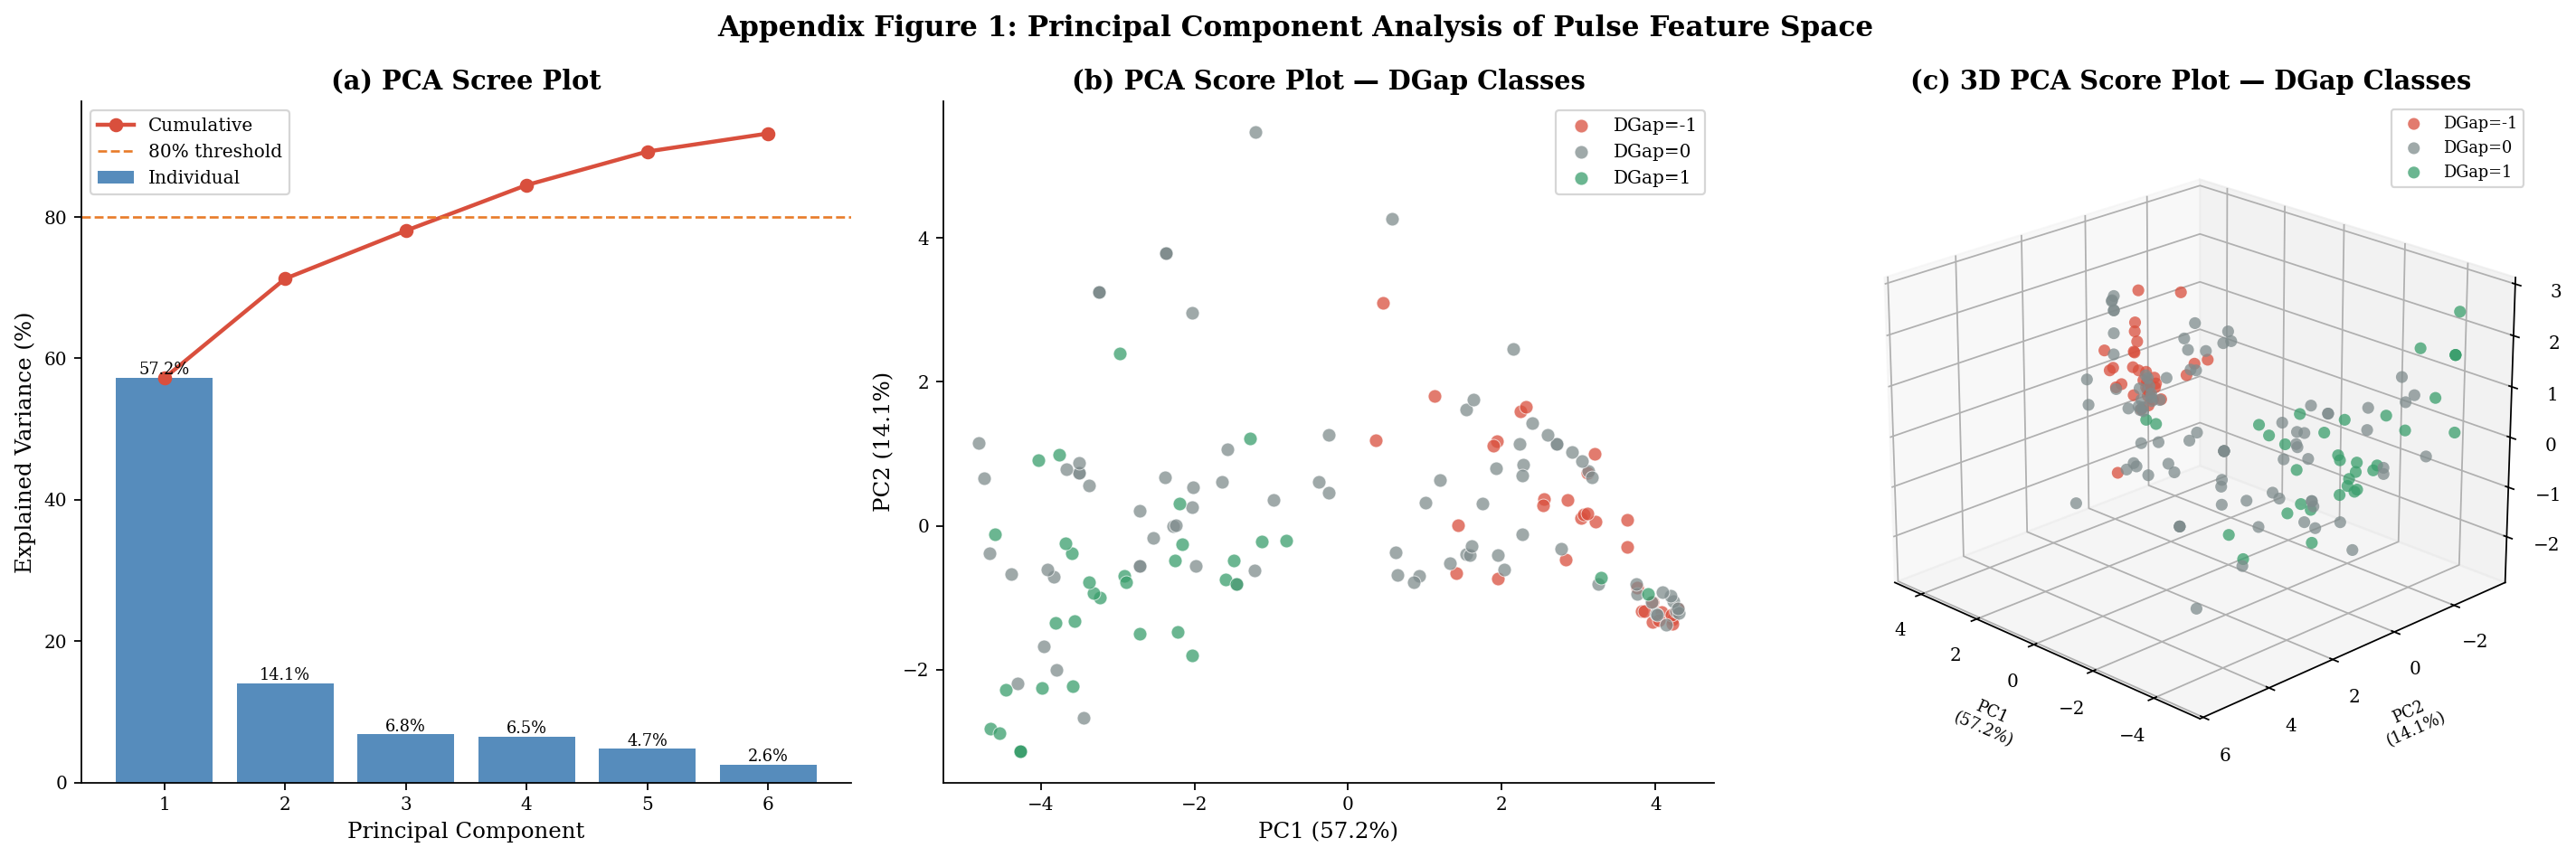
\includegraphics[width=\textwidth]{outputs/Fig3_PCA_Analysis.png}
\caption{附录图1：PCA 可视化结果。}
\label{fig:app_pca}
\end{figure}

\begin{figure}[H]
\centering
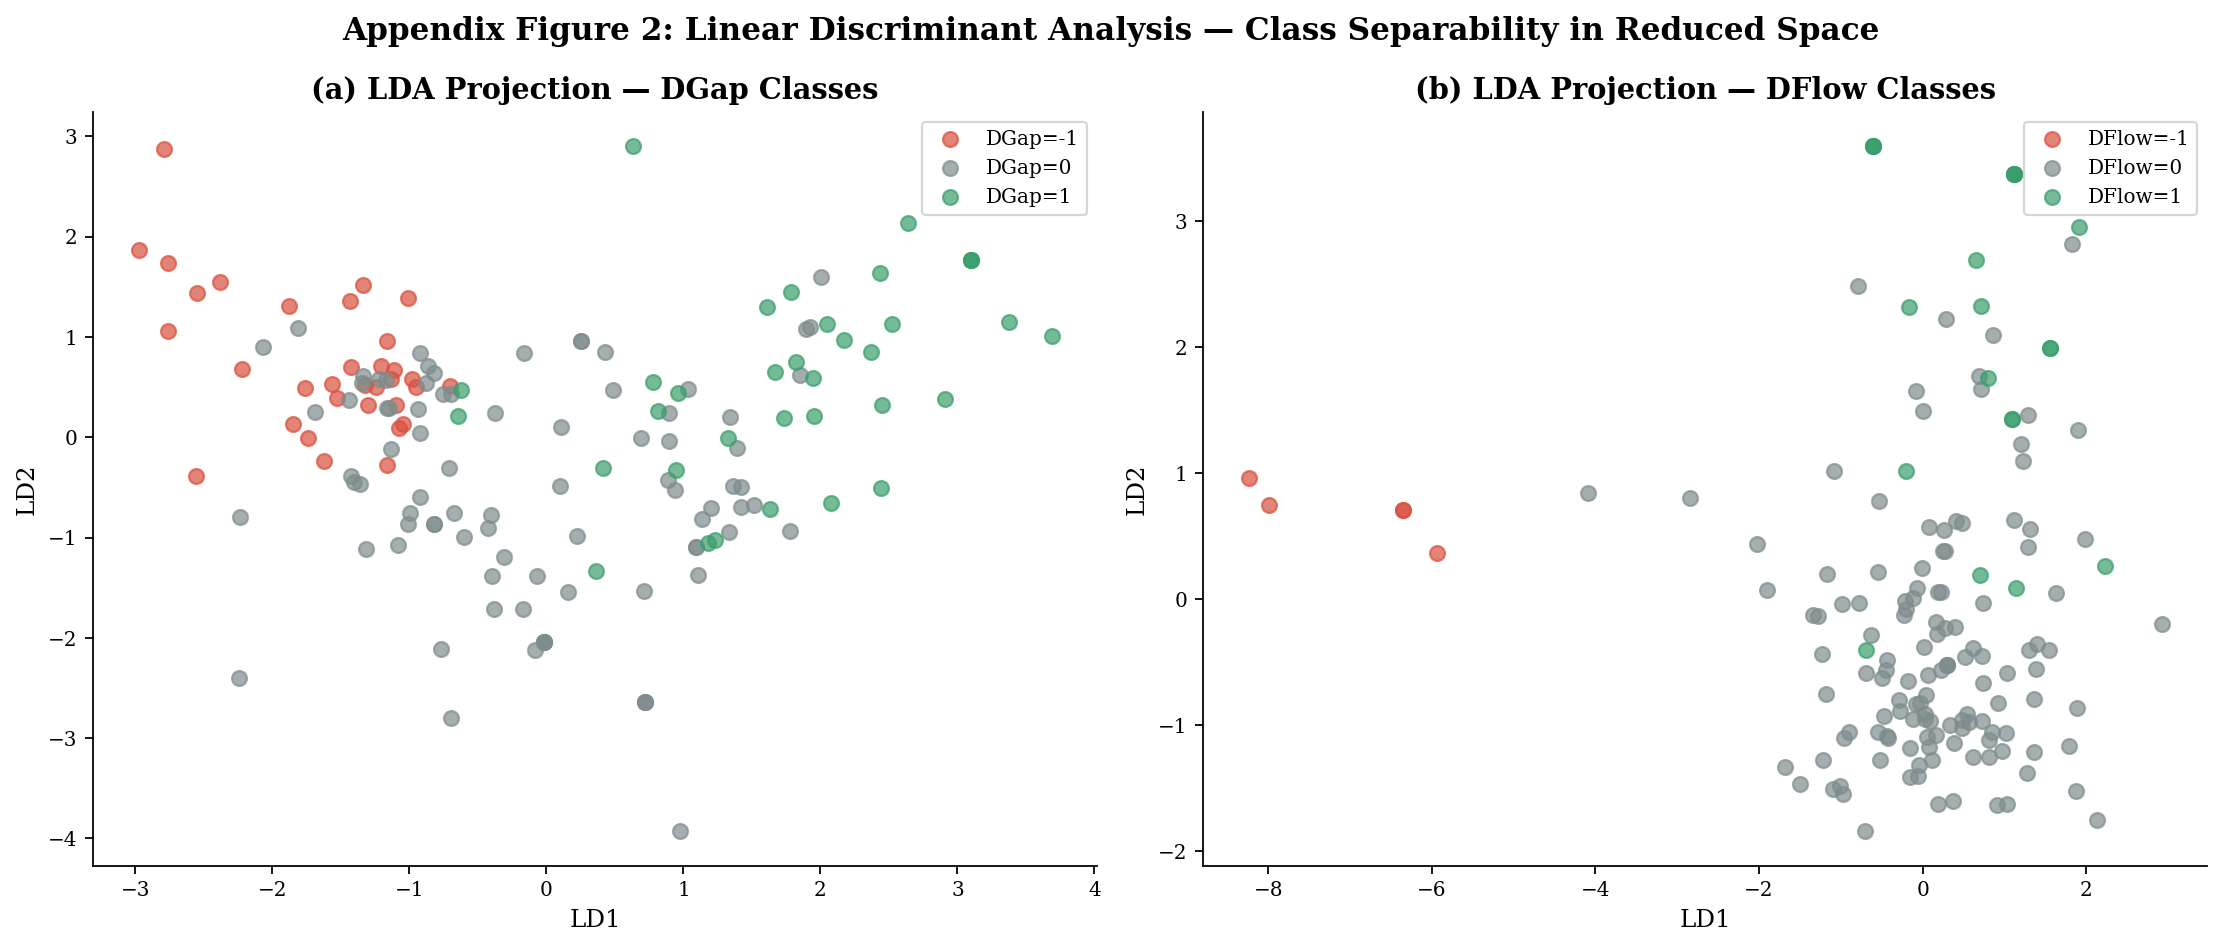
\includegraphics[width=0.92\textwidth]{outputs/Fig6_LDA_Analysis.png}
\caption{附录图2：LDA 判别结果。}
\label{fig:app_lda}
\end{figure}

\begin{figure}[H]
\centering
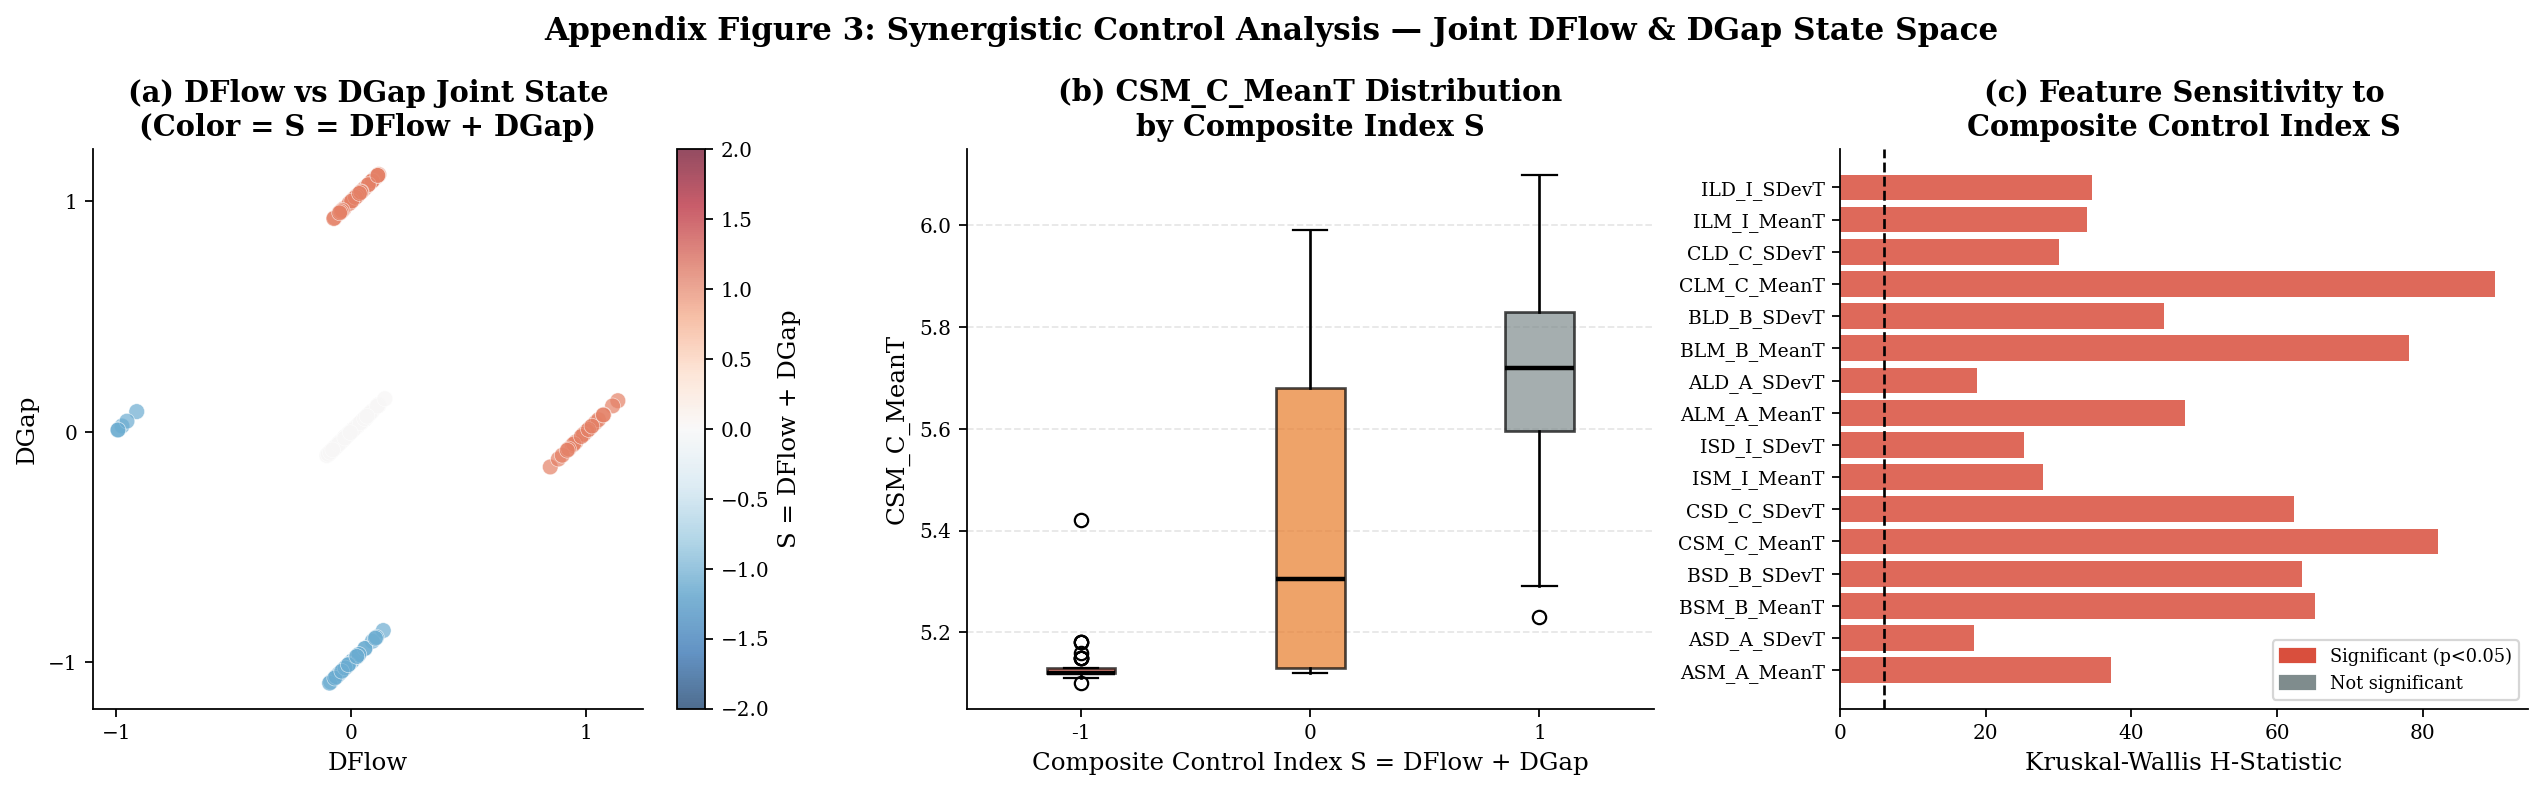
\includegraphics[width=\textwidth]{outputs/Fig9_Synergy_Analysis.png}
\caption{附录图3：联合状态与复合统计辅助分析。}
\label{fig:app_synergy}
\end{figure}

\section{建模代码}

由于本文采用了“双模型分类与协同调控”策略，且在验证环节进行了严格的数据防泄露处理，以下提供本文建模与求解的核心、完整、可运行的 Python 源程序代码（注：运行前需确保 ‘202601B题数据.xlsx’ 位于脚本同级目录）：

\begin{lstlisting}[language=Python]
import pandas as pd
import numpy as np
from scipy import stats
from scipy.cluster.hierarchy import linkage, fcluster
from sklearn.preprocessing import StandardScaler
from sklearn.pipeline import Pipeline
from sklearn.ensemble import RandomForestClassifier
from sklearn.svm import SVC
from sklearn.neighbors import KNeighborsClassifier
from sklearn.discriminant_analysis import LinearDiscriminantAnalysis
from sklearn.linear_model import LogisticRegression
from sklearn.model_selection import StratifiedKFold, train_test_split, cross_val_score
from sklearn.metrics import f1_score, accuracy_score, confusion_matrix, classification_report
from sklearn.base import clone
import warnings
warnings.filterwarnings('ignore')

# =====================================================================
# 1. 数据加载与基础处理
# =====================================================================
DATA_FILE = '202601B题数据.xlsx'
df = pd.read_excel(DATA_FILE)
features = [c for c in df.columns if c not in ['DFlow', 'DGap']]
X_raw = df[features].values
y_flow = df['DFlow'].values
y_gap = df['DGap'].values

print(f"[*] 数据加载完成: {df.shape[0]} 样本, {len(features)} 维度")

# =====================================================================
# 2. 层次聚类与特征精简 (消除多重共线性)
# =====================================================================
corr_mat = df[features].corr().abs()
dist_mat = 1 - corr_mat.values
np.fill_diagonal(dist_mat, 0)
Z_link = linkage(dist_mat, method='average')

# 在 d=0.4 (即 |r|>0.6) 处切割
cluster_labels = fcluster(Z_link, t=0.4, criterion='distance')
corr_dgap_abs = df[features].corrwith(df['DGap']).abs()

representative_features = []
for c in np.unique(cluster_labels):
    members = [features[i] for i, lbl in enumerate(cluster_labels) if lbl == c]
    # 选取与 DGap 相关性最强的特征作为该簇代表
    rep = corr_dgap_abs[members].idxmax()
    representative_features.append(rep)

X_reduced = df[representative_features].values
print(f"[*] 特征精简完成: 从 {len(features)} 维降至 {len(representative_features)} 维")
print(f"    代表特征: {representative_features}")

# =====================================================================
# 3. 构建防泄露的 Pipeline 及 5折交叉验证 (全特征 vs 精简特征)
# =====================================================================
def make_pipeline(clf):
    # 将标准化嵌入 Pipeline，确保仅在训练折拟合
    return Pipeline([('scaler', StandardScaler()), ('clf', clf)])

pipelines = {
    'Random Forest': make_pipeline(RandomForestClassifier(n_estimators=100, random_state=42, class_weight='balanced')),
    'SVM (RBF)': make_pipeline(SVC(kernel='rbf', C=10, gamma='scale', class_weight='balanced', random_state=42)),
    'k-NN (k=5)': make_pipeline(KNeighborsClassifier(n_neighbors=5)),
    'LDA': make_pipeline(LinearDiscriminantAnalysis()),
    'Logistic Reg': make_pipeline(LogisticRegression(max_iter=1000, class_weight='balanced', random_state=42))
}

cv5 = StratifiedKFold(n_splits=5, shuffle=True, random_state=42)

print("\n[*] 开始 5 折交叉验证模型评估 (Pipeline Macro-F1)...")
for name, pipe in pipelines.items():
    f1_flow_all = cross_val_score(pipe, X_raw, y_flow, cv=cv5, scoring='f1_macro') * 100
    f1_gap_all = cross_val_score(pipe, X_raw, y_gap, cv=cv5, scoring='f1_macro') * 100
    if name in ['Random Forest', 'SVM (RBF)']:
        print(f"    {name:<15} | DFlow F1: {f1_flow_all.mean():.1f}% | DGap F1: {f1_gap_all.mean():.1f}%")

# =====================================================================
# 4. 协同调控：分类器链 (Classifier Chain) 模型实现
# =====================================================================
def classifier_chain_cv(X, y_first, y_second, base_first, base_second, cv):
    scores_joint = []
    for train_idx, test_idx in cv.split(X, y_first):
        X_train, X_test = X[train_idx], X[test_idx]
        y_first_train, y_first_test = y_first[train_idx], y_first[test_idx]
        y_second_train, y_second_test = y_second[train_idx], y_second[test_idx]

        clf_first, clf_second = clone(base_first), clone(base_second)

        # 1. 训练第一级分类器并预测
        clf_first.fit(X_train, y_first_train)
        first_test_pred = clf_first.predict(X_test)

        # 2. 将第一级的真实/预测标签作为特征拼接，训练第二级
        X_train_chain = np.column_stack([X_train, y_first_train])
        X_test_chain = np.column_stack([X_test, first_test_pred])
        
        clf_second.fit(X_train_chain, y_second_train)
        second_test_pred = clf_second.predict(X_test_chain)

        # 3. 评估联合状态
        joint_true = [f"{a}_{b}" for a, b in zip(y_first_test, y_second_test)]
        joint_pred = [f"{a}_{b}" for a, b in zip(first_test_pred, second_test_pred)]
        scores_joint.append(f1_score(joint_true, joint_pred, average='macro'))
        
    return np.array(scores_joint) * 100

chain_rf = pipelines['Random Forest']
chain_svm = pipelines['SVM (RBF)']

print("\n[*] 运行分类器链 (协同调控) 评估...")
chain_flow_gap = classifier_chain_cv(X_raw, y_flow, y_gap, chain_rf, chain_svm, cv5)
chain_gap_flow = classifier_chain_cv(X_raw, y_gap, y_flow, chain_svm, chain_rf, cv5)

print(f"    顺序 [DFlow -> DGap] 联合 Macro-F1 = {chain_flow_gap.mean():.1f}%")
print(f"    顺序 [DGap -> DFlow] 联合 Macro-F1 = {chain_gap_flow.mean():.1f}%")

# =====================================================================
# 5. 最终双模型策略测试集评估 (问题三)
# =====================================================================
# 统一划分测试集，按更不均衡的 DFlow 分层抽样
idx_all = np.arange(len(y_flow))
idx_tr, idx_te = train_test_split(idx_all, test_size=0.25, random_state=42, stratify=y_flow)

X_tr, X_te = X_raw[idx_tr], X_raw[idx_te]
yf_tr, yf_te = y_flow[idx_tr], y_flow[idx_te]
yg_tr, yg_te = y_gap[idx_tr], y_gap[idx_te]

# DFlow 采用 Random Forest, DGap 采用 SVM (RBF)
pipe_rf_final = make_pipeline(RandomForestClassifier(n_estimators=300, random_state=42, class_weight='balanced'))
pipe_svm_final = make_pipeline(SVC(kernel='rbf', C=10, gamma='scale', class_weight='balanced', random_state=42))

pipe_rf_final.fit(X_tr, yf_tr)
pipe_svm_final.fit(X_tr, yg_tr)

yf_pred = pipe_rf_final.predict(X_te)
yg_pred = pipe_svm_final.predict(X_te)

print("\n[*] 最终双模型测试集评估结果:")
print(f"    DFlow (RF Model) Macro-F1: {f1_score(yf_te, yf_pred, average='macro')*100:.1f}%")
print(f"    DGap (SVM Model) Macro-F1: {f1_score(yg_te, yg_pred, average='macro')*100:.1f}%")

print("\n[DFlow 详细分类报告]")
print(classification_report(yf_te, yf_pred, target_names=['DFlow=-1', 'DFlow=0', 'DFlow=+1']))
print("[DGap 详细分类报告]")
print(classification_report(yg_te, yg_pred, target_names=['DGap=-1', 'DGap=0', 'DGap=+1']))
\end{lstlisting}

\end{document}
